
\chapter{Vergleichende Anatomie}
\label{appendix_vergleichende_anatomie}

Notizen aus "`Vergleichende und funktionelle Anatomie der Wirbeltiere"' \cite{Vergleichende_Anatomie}:\\

\textbf{Kapitel 1} - Einleitung
\begin{itemize}
 \item "`Nichts anderes in der Natur hat eine herrlichere Struktur als der Körper der Wirbeltiere."' (S.\ 1)
 \item Anpassung des Körpers an äußere Gegebenheiten (S.\ 3). $\rightarrow$ Eingabeparameter?
 \item (phylogenetische) Homologie von Strukturen: gemeinsame Abstammung (meist auch gleiche Funktion) (S.\ 4 und 6)
 \item Analogie von Strukturen: gleiche Funktion aber nicht gleiche phylogenetische Herkunft (S.\ 6)
 \item serielle Homologie: homologe Gene an verschiedenen Körperteilen aktiviert (\zb Wirbel) (S.\ 7) $\rightarrow$ gleiche/sehr ähnliche Regeln
 \item rudimentäre/degenerierte Organe: haben keine Funktion mehr, waren aber bei Vorfahren funktionell (\zb Beckengürtel des Finnwals) (S.\ 9/10)
 \item Veränderungen von Körperproportionen (\zb Schädelknochen) können durch eine fortschreitende Verzerrung eines Gitters beschrieben werden (S.\ 18/19), siehe auch  Anhang \ref{appendix_darcy_thompson}
\end{itemize}

\textbf{Kapitel 2} - Charakterisierung , Ursprung und Einteilung der Vertebraten
\begin{itemize}
 \item "`[\dots] ein Tier mit einem Cranium, also einer skelettartigen Schädelkapsel, [ist] ein Vertebrat."' (S.\ 27)
 \item Teil der allgeime Beschreibung der (meisten) Vertebraten (S.\ 27): 
 \begin{itemize}
  \item "`Der Körper ist bilateralsymmetrisch, \dash er weist eine rechte und eine linke Seite, ein anteriores und ein posteriores Ende und eine dorsale und eine ventrale Oberfläche auf."'
  \item Sie haben ein inneres Skelett.
 \end{itemize}
\end{itemize}

\textbf{Kapitel 3} - Fische
\begin{itemize}
 \item Agnathen (Kieferlose): erste bekannte Vertebraten und einzige ohne Kiefer. Einzige rezente Arten: Neunauge und Schleimaal (S.\ 41/42)
 \item Kiefertragende Fische: 1.\ Kiemenbogen entwickelte sich zu Kiefer, haben paarige Flossen (S.\ 45/46)
 \begin{itemize}
  \item Knorpelfische: Haie, Rochen, Chimären; verkalkte Knorpel aber wenige/keine Knochen (S.\ 47) (Unterschied Knochen/Knorpel ignorieren oder nur Knochenfischskelette generieren?)
  \item Knochenfische: Strahlenflosser (Flossen mit knöchernen Strahlen), Fleischflosser (Flossen mit fleischigen Stielen) (S.\ 52/53)
 \end{itemize}
\end{itemize}

\textbf{Kapitel 4} - Tetrapoden
\begin{itemize}
 \item an Land ist Stromlinienform und sind Flossen kein Vorteil mehr, ein Hals ist nützlich und der Körper muss von Beinen getragen werden $\rightarrow$ Extremitätengürtel fester mit Axialskelett verbunden (S.\ 59)
 \item Amphibien: nicht vollkommen terrestrisch (Haut feucht, Eier im Wasser / feucht). Unterklasse Lissamphibia (dazu gehören alle rezenten Amphibien) haben nur vier Zehen am Vorderfuß. Es gibt drei Ordnungen: Anura (Schwanzlose), Urodela (Schwanzlurche) und Apoda (Beinlose) (S.\ 61)
 \item Reptilien: erste Klasse mit allen Strukturen für vollkommen landgebundenes Leben, leben aber auch teilweise wieder im Wasser (S.\ 62)
 \item Vögel: alle rezenten Vögel fliegen oder sind Nachkommen von Fliegern. Erste Zehe ist opponiert (siehe Diagramm S.\ 71). (S.\ 67)
 \item Säugetiere (S.\ 71 f)
\end{itemize}

\textbf{Kapitel 8} - (Kopfskelett)
\begin{itemize}
 \item "`Das innere, gelenkige Skelettsystem der Vertebraten ist einzigartig im Tierreich. Es ist das wichtigste aller Organsysteme für das Studium der Wirbeltiermorphologie."' (S.\ 131)
 \item Muskeln haben Ansatzstellen an Knochen, die Lage und Ausmaße zeigen. (S.\ 131)
\end{itemize}

\textbf{Kapitel 9} - Körperskelett
\begin{itemize}
 \item "`Die Wirbelsäule ist älter als jeder andere Teil des postcranialen Skeletts mit Ausnahme der Chorda dorsalis. Dennoch ist sie nicht so alt wie die Hauptmerkmale der weichen Organsysteme, und sie fehlt praktisch bei den ältesten, bekannten Vertebraten."' (S.\ 163)
 \item Wirbel können viele verschiedene Merkmale haben, \zb Dornfortsatz, Ansatz der Rippe (siehe Bild S.\ 165) (S.\ 163)
 \item Evolution der Wirbelsäule: zunächst Chorda dorsalis mit stützenden Knorpeln (S.\ 166)
 \item Rippen
 \begin{itemize}
  \item ursprünglich über die gesamte Länge der Wirbelsäule vorhanden. Zwei Arten: Dorsalrippen und Ventralrippen (siehe Abb.\ S.\ 173) (S.\ 172)
  \item keine Rippen bei kieferlosen Vertebraten und Placodermi
 \end{itemize}
 \item Mediane Flossen (175 f)
 \begin{itemize}
  \item Dorsalflosse, Analflosse und Schwanzflosse
  \item treten bei fast allen Agnatha und kiefertragenden Fischen auf
  \item Wirbelsäule kann unterschiedlich in Schwanzflosse liegen (gerade, nach oben/unten geknickt oder sie hört davor auf), meistens nach oben abgeknickt (heterocerk).
 \end{itemize}
 \item Schultergürtel der Fische ist mit Kopf verbunden (S.\ 178) (also kein Hals)
 \item Beckengürtel der Tetrapoden viel größer als bei Fischen. Bei verschiednene Gruppen unterschiedlich aber speziell (\zb Vogel, Säugetier,\dots) (S.\ 180 f) $\rightarrow$ diskret repräsentieren?
 \item S.\ 183 Abbildung zur Evolution der Vordergliedmaßen
 \item Amphibien haben meistens kurze Gliedmaßen, die seitlich des Körpers nach außen gestellt sind (S.\ 187)
 \item Gliedmaßen der Reptilien oft seitlich aber manche auch unter dem Körper (wie bei Säugetieren) (S.\ 188 f)
\end{itemize}

\textbf{Kapitel 21} - Strukturelemente des Körpers
\begin{itemize}
 \item "`allgemein nützliche"' Strukturen: Kiefer, zwei Paare von Extremitäten (S.\ 433)
 \item Skelett kann nicht einfach "`groß skaliert"' werden. Belastung ist sonst möglicherweise zu groß (S.\ 444, siehe auch S.\ 478 und S.\ 481)
 \item Knochen halten am besten Druckkraft aus $\rightarrow$ Minimierung anderer Kräfte (S.\ 444)(schlecht bei Zug oder seitlicher Belastung)
\end{itemize}

\textbf{Kapitel 22} - Mechanik von Stützung und Bewegung\\
\begin{itemize}
 \item Balance und Gegenmoment (S.\ 466)
\end{itemize}


%--------------
\chapter{D'Arcy Thompson}
\label{appendix_darcy_thompson}

(siehe auch \url{https://en.wikipedia.org/wiki/On_Growth_and_Form})

Notizen aus "`Über Wachstum und Form"' von D'Arcy Wentworth Thompson \cite{DArcy_Thompson}:\\

\textbf{Kapitel 2} - Über die Größe
\begin{itemize}
 \item Maximale und minimale Größe eines Tieres sind durch unterschiedliche Faktoren, wie \zb das Atmungssystem festgelegt. Bei Säugetieren: min.\ 5g (Maus)  (S.\ 68) und max.\ sowas wie Elefant
\end{itemize}

\textbf{Kapitel 4} - Über die Theorie der Transformationen oder den Vergleich verwandter Formen
\begin{itemize}
 \item "`Es handelt sich hier um das berühmteste Kapitel des Buches, das in der biologischen Literatur schon vielfach besprochen worden ist."' (S.\ 325, Kommentar des Herausgebers (?))
 \item Kartesische Transormationen (S.\ 334 ff)
 \begin{enumerate}
  \item entlang einer Achse ausdehnen
  \item logarithmische Verlängerung
  \item einfache Scherung
  \item radiale Koordinaten
 \end{enumerate}
 \item Beispiele \zb S.\ 366 f, Säugetierschädel ab S.\ 371
\end{itemize}


%-------------------------------
\chapter{Erhobene Daten für PCA}
\label{appendix_pca}
 
  \begin{figure}
   \subfloat[Erster Punkt des Halses]{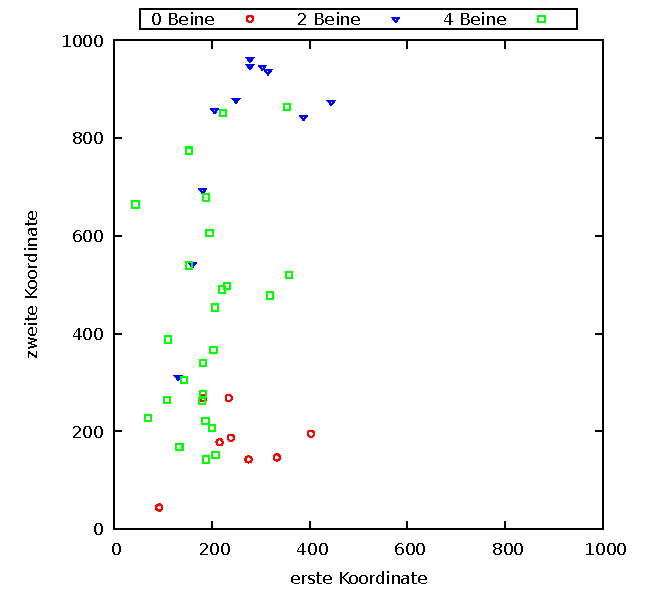
\includegraphics[width=0.3\textwidth]{../PCA/gnuplot/results_with_leg_tag/input_neck1.pdf}}
   \qquad
   \subfloat[Zweiter Punkt des Halses]{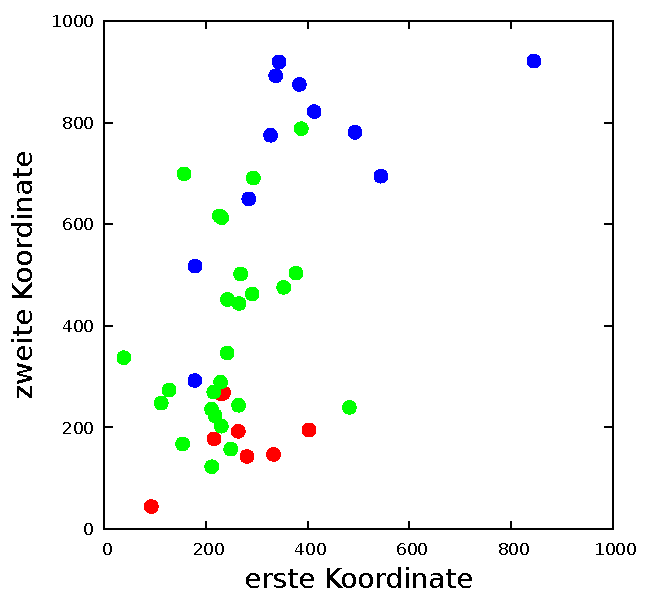
\includegraphics[width=0.3\textwidth]{../PCA/gnuplot/results_with_leg_tag/input_neck2.pdf}}
   \qquad
   \subfloat[Dritter Punkt des Halses]{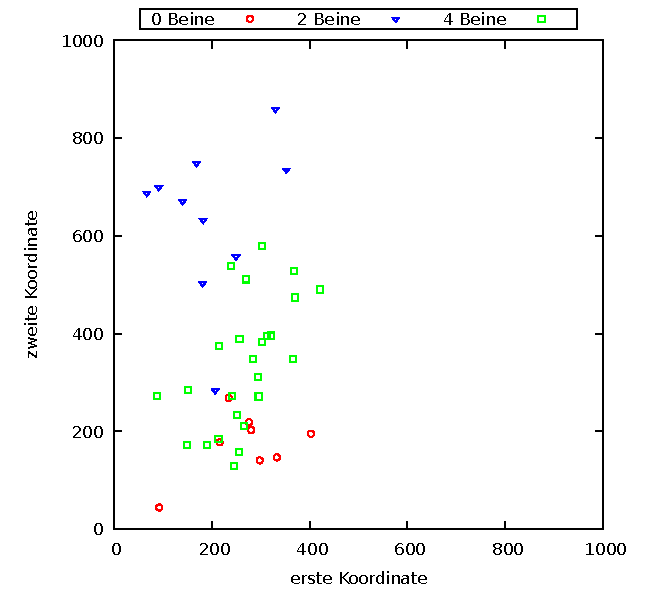
\includegraphics[width=0.3\textwidth]{../PCA/gnuplot/results_with_leg_tag/input_neck3.pdf}}
   \\
   \subfloat[Vierter Punkt des Halses \bzw erster Punkt des Rückens]{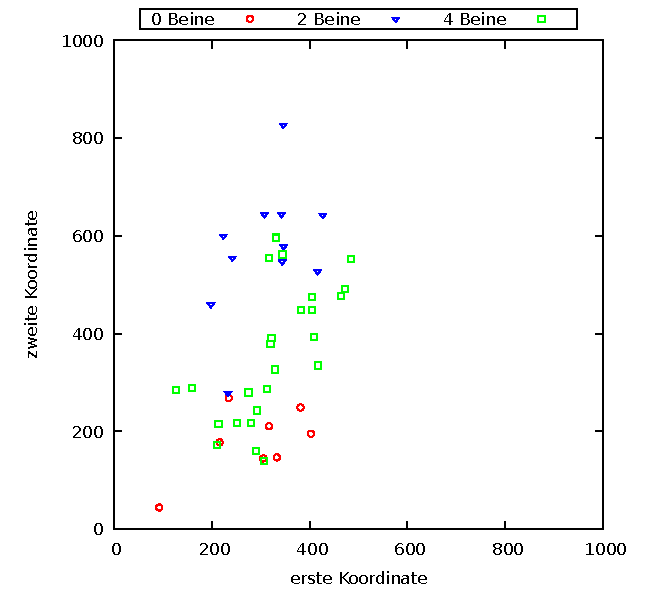
\includegraphics[width=0.3\textwidth]{../PCA/gnuplot/results_with_leg_tag/input_back1.pdf}}
   \qquad
   \subfloat[Zweiter Punkt des Rückens]{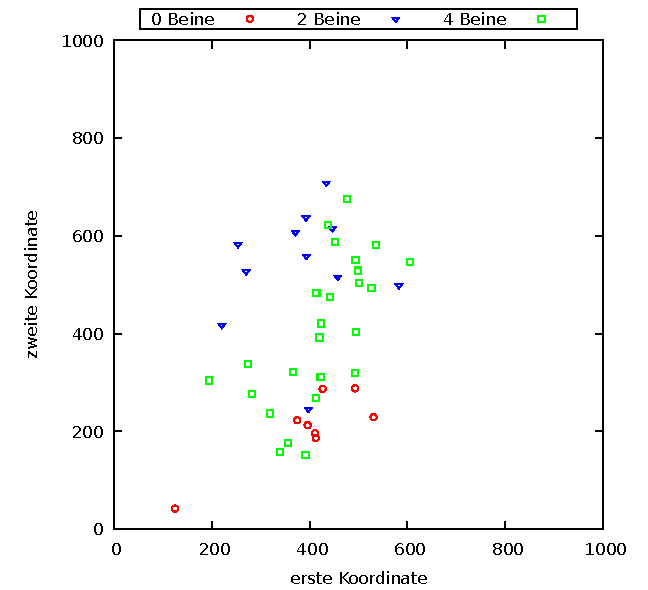
\includegraphics[width=0.3\textwidth]{../PCA/gnuplot/results_with_leg_tag/input_back2.pdf}}
   \qquad
   \subfloat[Dritter Punkt des Rückens]{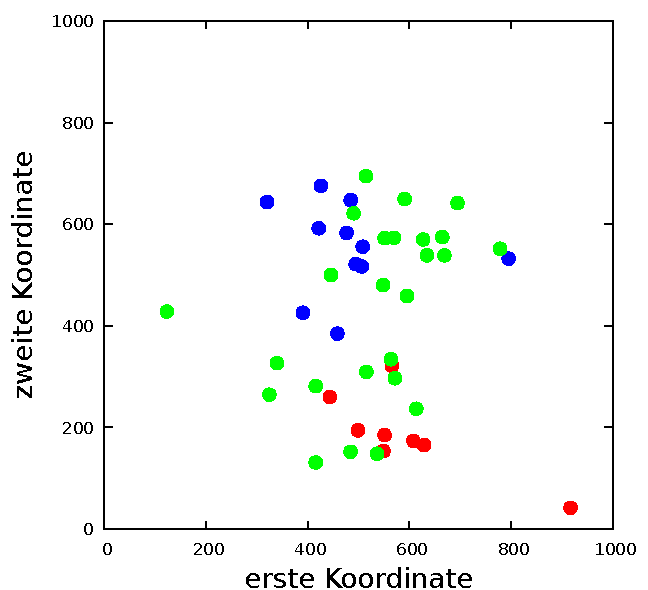
\includegraphics[width=0.3\textwidth]{../PCA/gnuplot/results_with_leg_tag/input_back3.pdf}}
   \\
   \subfloat[Vierter Punkt des Rückens \bzw erster Punkt des Schwanzes]{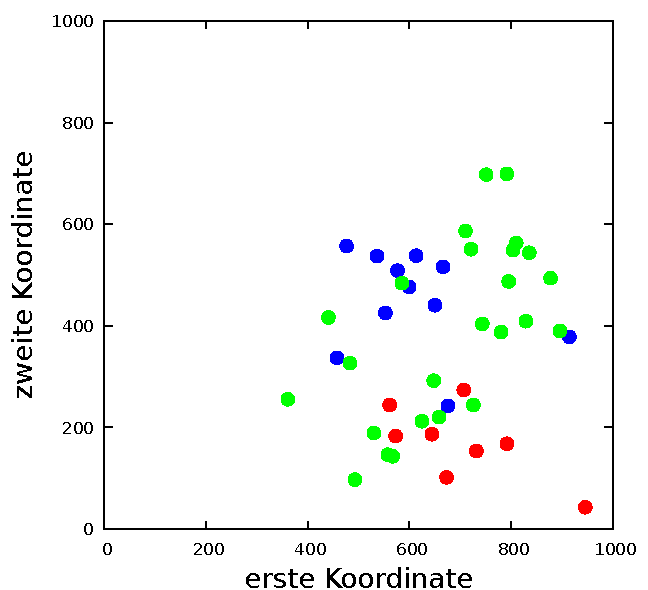
\includegraphics[width=0.3\textwidth]{../PCA/gnuplot/results_with_leg_tag/input_back4.pdf}}
   \qquad
   \subfloat[Zweiter Punkt des Schwanzes]{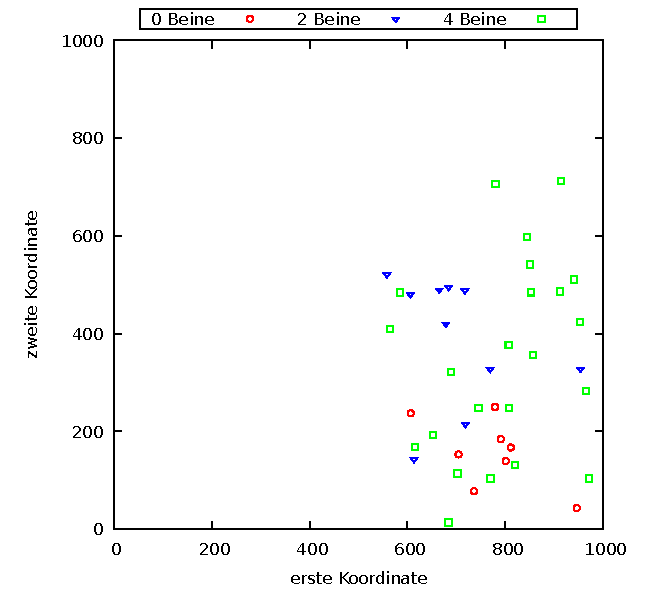
\includegraphics[width=0.3\textwidth]{../PCA/gnuplot/results_with_leg_tag/input_tail2.pdf}}
   \qquad
   \subfloat[Dritter Punkt des Schwanzes]{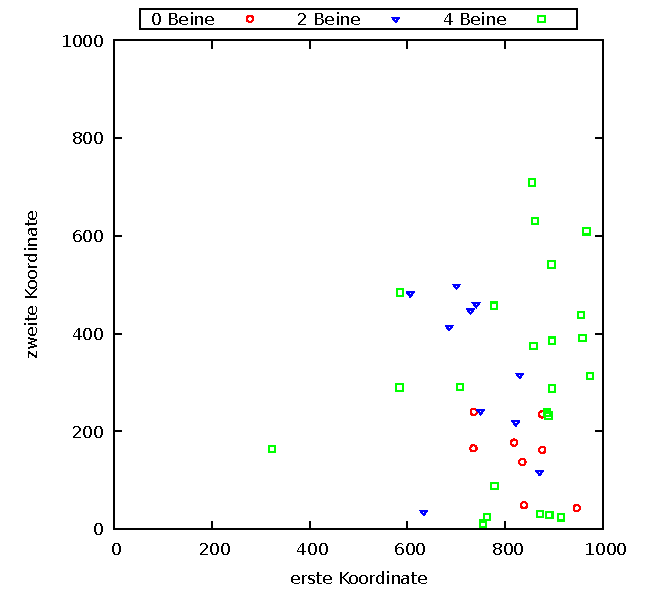
\includegraphics[width=0.3\textwidth]{../PCA/gnuplot/results_with_leg_tag/input_tail3.pdf}}
   \\
   \subfloat[Vierter Punkt des Schwanzes]{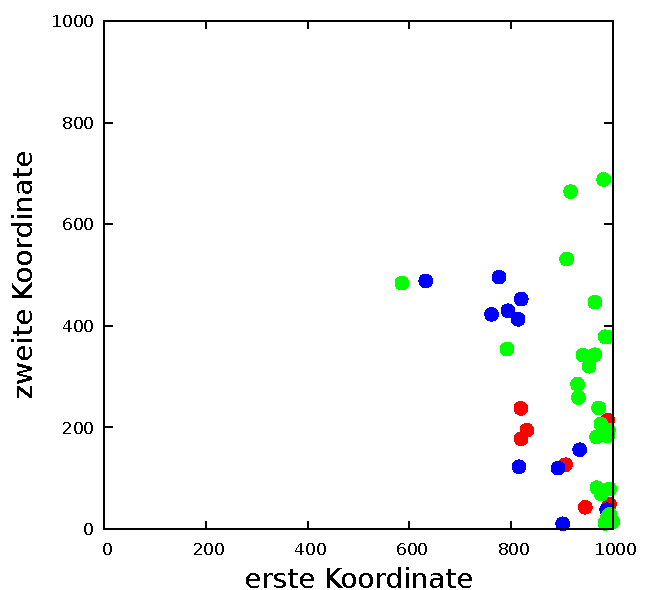
\includegraphics[width=0.3\textwidth]{../PCA/gnuplot/results_with_leg_tag/input_tail4.pdf}}
   \qquad
   \subfloat[Länge Ober- und Unterarm]{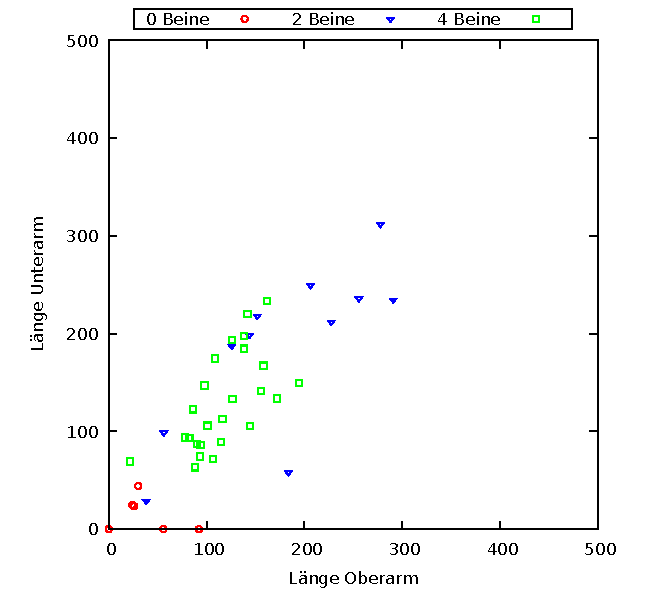
\includegraphics[width=0.3\textwidth]{../PCA/gnuplot/results_with_leg_tag/input_upper+lowerArm.pdf}}
   \qquad
   \subfloat[Länge Unterarm und Hand]{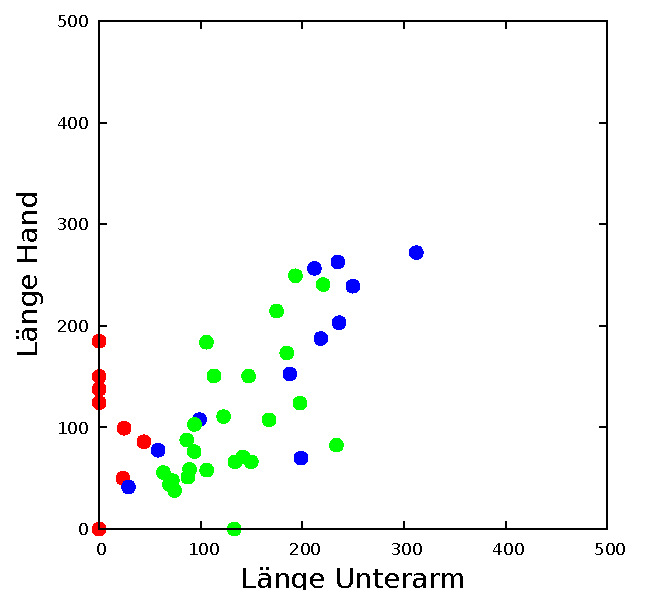
\includegraphics[width=0.3\textwidth]{../PCA/gnuplot/results_with_leg_tag/input_lowerArm+hand.pdf}}
   \phantomcaption
  \end{figure}
  \begin{figure}
   \ContinuedFloat
   \subfloat[Länge Ober- und Unterschenkel]{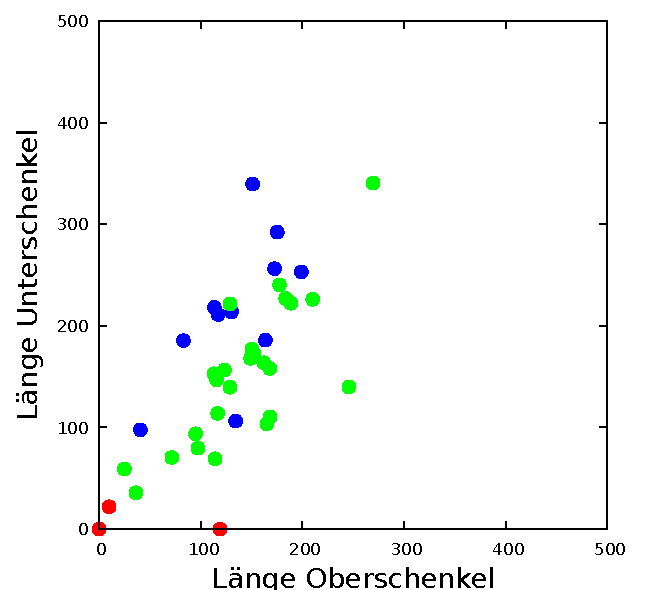
\includegraphics[width=0.3\textwidth]{../PCA/gnuplot/results_with_leg_tag/input_upper+lowerLeg.pdf}}
   \qquad
   \subfloat[Länge Unterschenkel und Fuß]{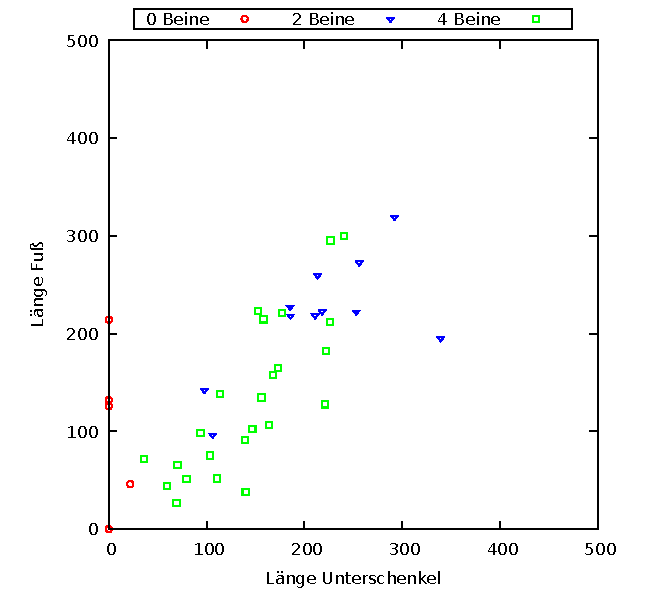
\includegraphics[width=0.3\textwidth]{../PCA/gnuplot/results_with_leg_tag/input_lowerLeg+foot.pdf}}
   
   \caption{Erhobene Daten: Punkte der Bézierkurven der Wirbelsäule und Längen der Extremitäten. Bei den Extremitäten ist jeweils gegeneinander abgetragen Ober- und Unterarm, Ober- und Unterschenkel, Unterarm und Hand, Unterschenkel und Fuß. Markiert ist jeweils ob die Datenpunkte $0$ (rot), $2$ (blau) oder $4$ (grün) Beine haben.}
   \label{input_data}
  \end{figure}
  
 \begin{figure}
  \subfloat[lineare Skala]{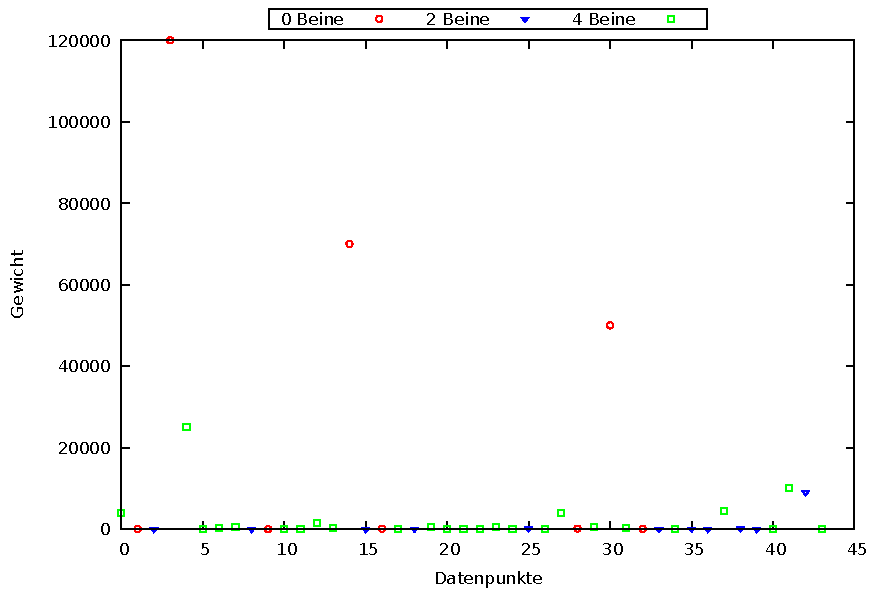
\includegraphics[width=0.5\textwidth]{../PCA/gnuplot/results_with_leg_tag/input_weight.pdf} \label{gnuplot_weight}}
  \qquad
  \subfloat[logarithmische Skala]{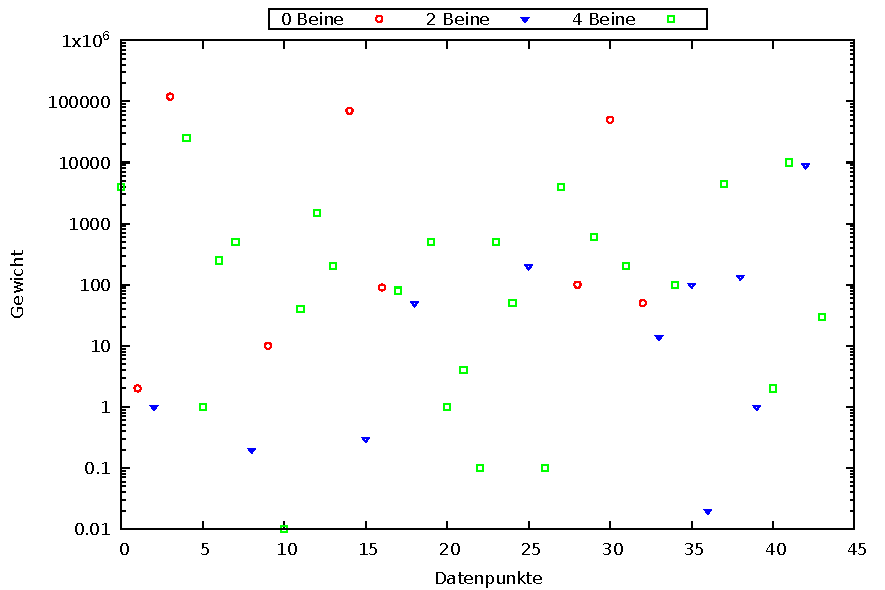
\includegraphics[width=0.5\textwidth]{../PCA/gnuplot/results_with_leg_tag/input_weight_logarithmic.pdf}\label{gnuplot_log_weight}}
  
  \caption{Erhobene Daten: Gewicht. Markiert ist jeweils ob die Datenpunkte $0$ (rot), $2$ (blau) oder $4$ (grün) Beine haben.}
  \label{input_data_weight}
 \end{figure}
 
 %--------------
 % QQ Diagramme
 % ------------

  \begin{figure}
   \subfloat[Erster Punkt des Halses, x-Koordinate]{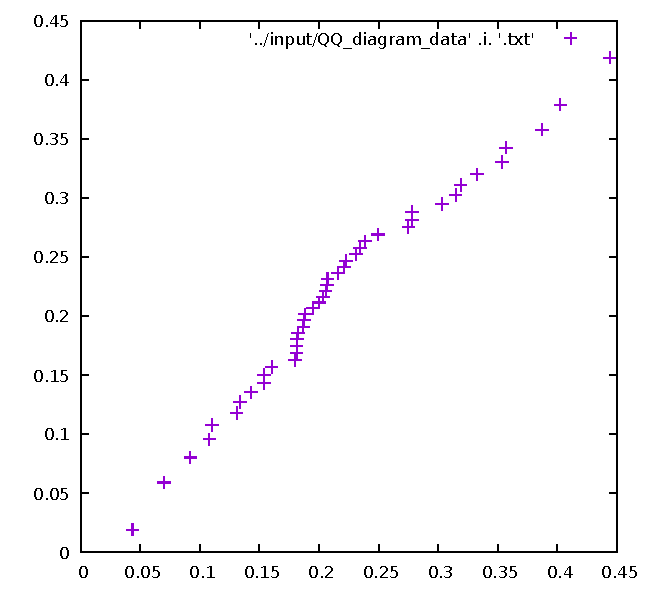
\includegraphics[width=0.3\textwidth]{../PCA/gnuplot/results_qq_diagrams/QQ_diagram0.pdf}}
   \qquad
   \subfloat[Erster Punkt des Halses, y-Koordinate]{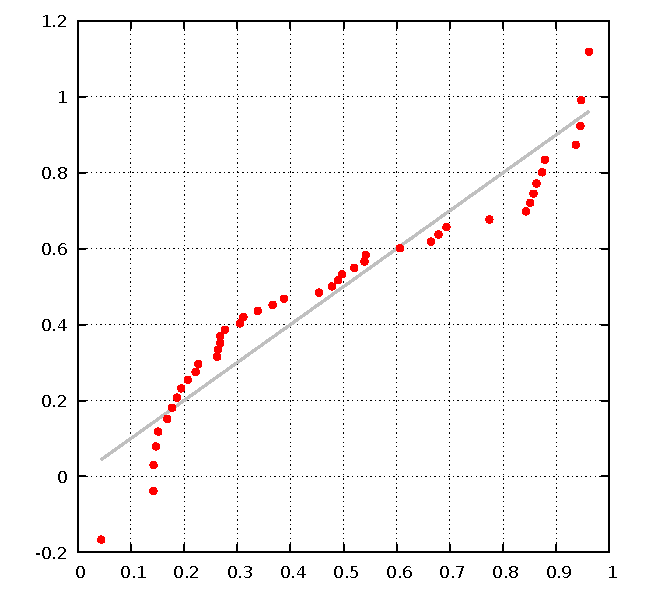
\includegraphics[width=0.3\textwidth]{../PCA/gnuplot/results_qq_diagrams/QQ_diagram1.pdf}}
   \qquad
   \subfloat[Zweiter Punkt des Halses, x-Koordinate]{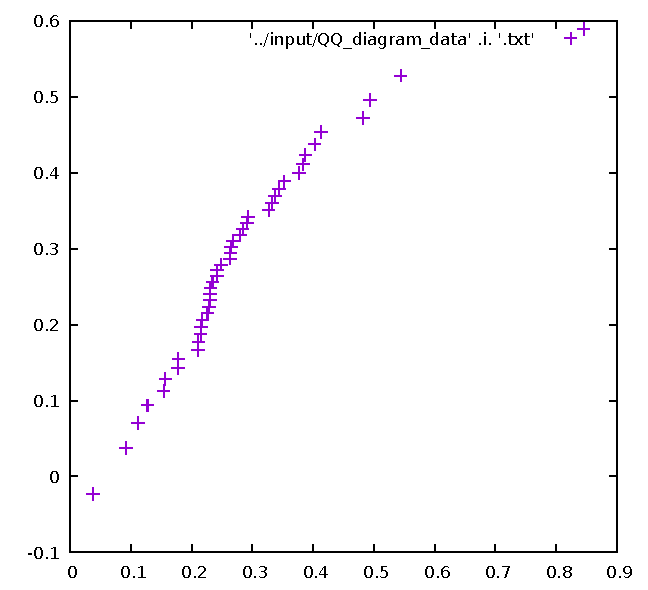
\includegraphics[width=0.3\textwidth]{../PCA/gnuplot/results_qq_diagrams/QQ_diagram2.pdf}}
   \\
   \subfloat[Zweiter Punkt des Halses, y-Koordinate]{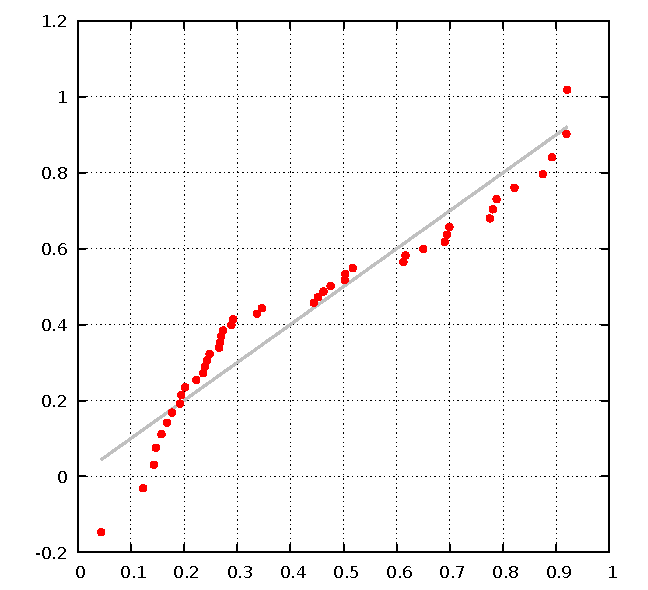
\includegraphics[width=0.3\textwidth]{../PCA/gnuplot/results_qq_diagrams/QQ_diagram3.pdf}}
   \qquad
   \subfloat[Dritter Punkt des Halses, x-Koordinate]{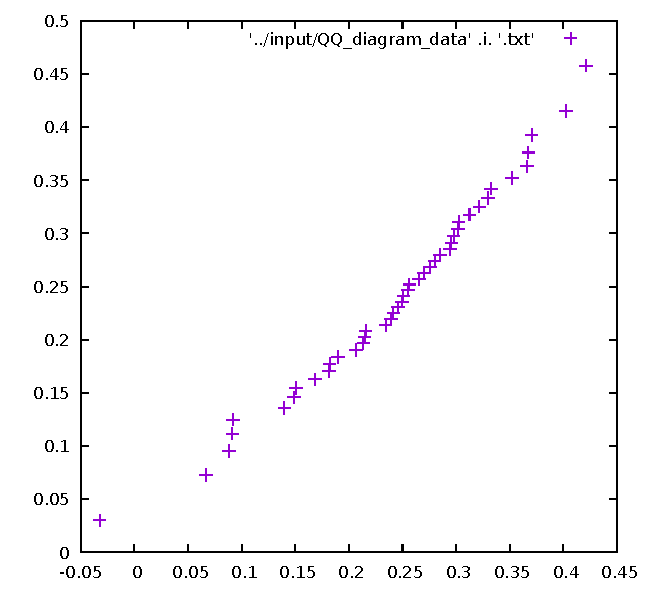
\includegraphics[width=0.3\textwidth]{../PCA/gnuplot/results_qq_diagrams/QQ_diagram4.pdf}}
   \qquad
   \subfloat[Dritter Punkt des Hales, y-Koordinate]{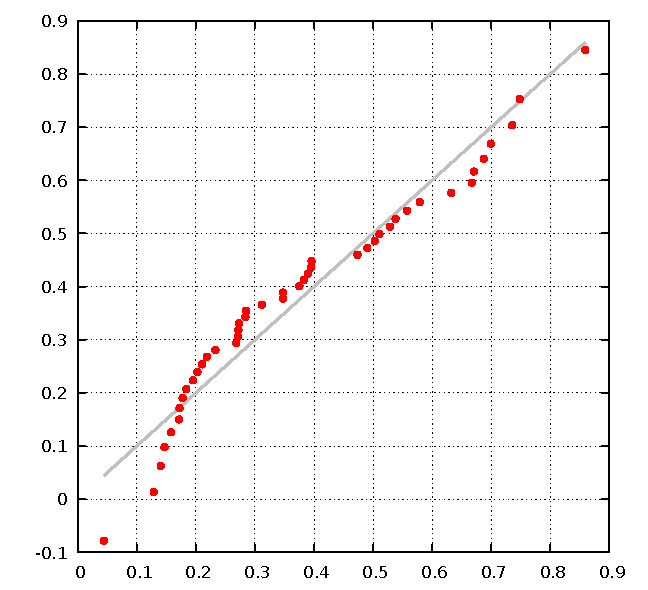
\includegraphics[width=0.3\textwidth]{../PCA/gnuplot/results_qq_diagrams/QQ_diagram5.pdf}}
   \\
   \subfloat[Erster Punkt des Rückens, x-Koordinate]{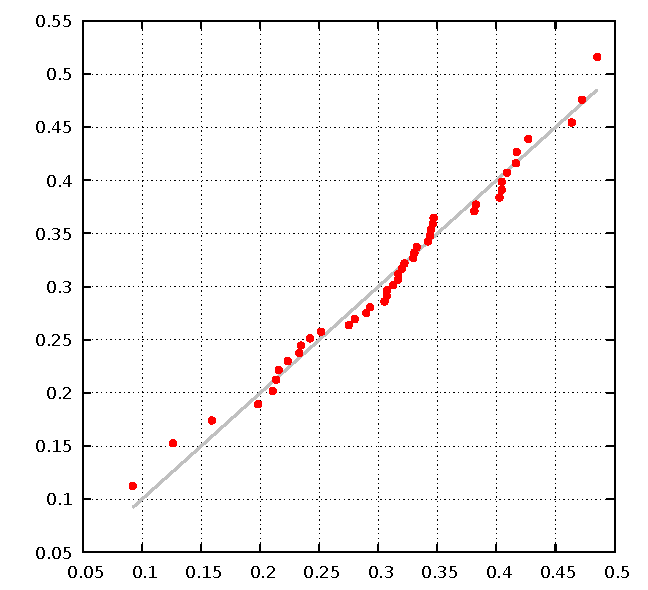
\includegraphics[width=0.3\textwidth]{../PCA/gnuplot/results_qq_diagrams/QQ_diagram6.pdf}}
   \qquad
   \subfloat[Erster Punkt des Rückens, y-Koordinate]{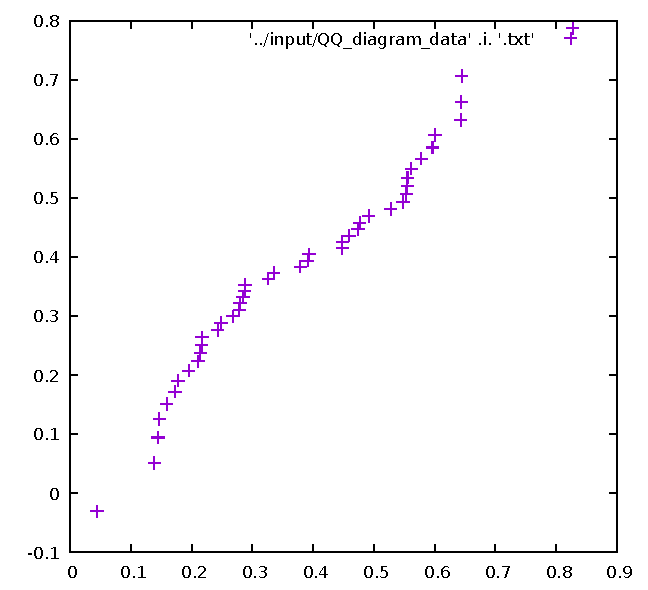
\includegraphics[width=0.3\textwidth]{../PCA/gnuplot/results_qq_diagrams/QQ_diagram7.pdf}}
   \qquad
   \subfloat[Zweiter Punkt des Rückens, x-Koordinate]{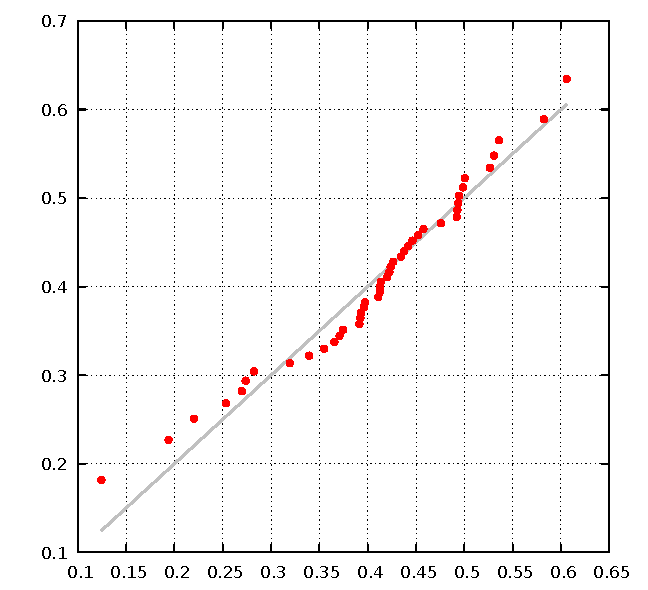
\includegraphics[width=0.3\textwidth]{../PCA/gnuplot/results_qq_diagrams/QQ_diagram8.pdf}}
   \\
   \subfloat[Zweiter Punkt des Rückens, y-Koordinate]{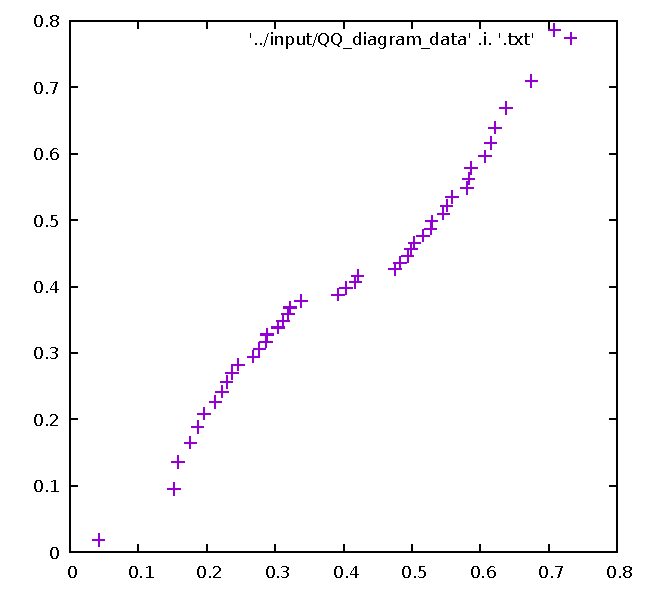
\includegraphics[width=0.3\textwidth]{../PCA/gnuplot/results_qq_diagrams/QQ_diagram9.pdf}}
   \qquad
   \subfloat[Dritter Punkt des Rückens, x-Koordinate]{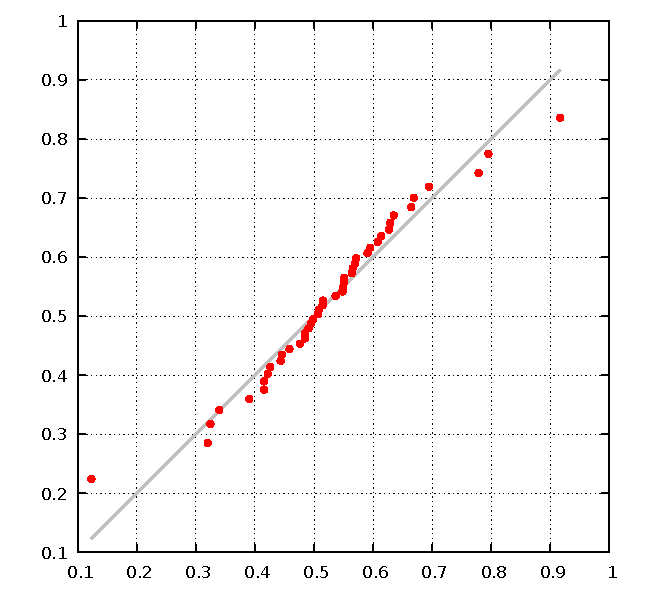
\includegraphics[width=0.3\textwidth]{../PCA/gnuplot/results_qq_diagrams/QQ_diagram10.pdf}}
   \qquad
   \subfloat[Dritter Punkt des Rückens, y-Koordinate]{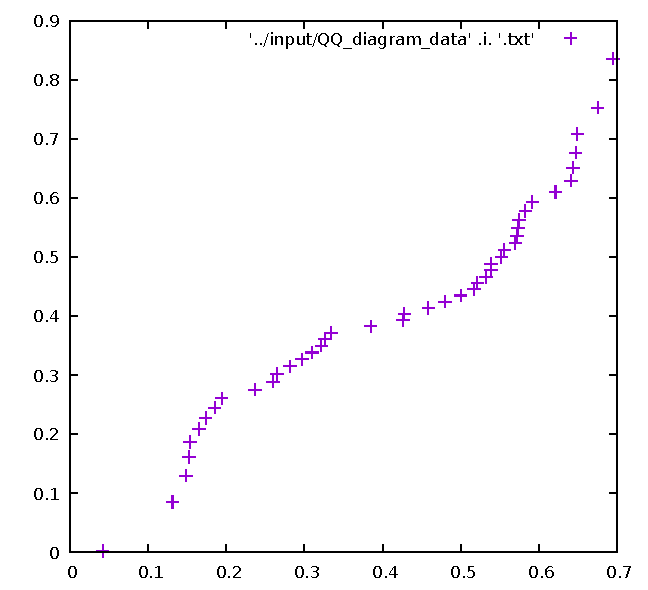
\includegraphics[width=0.3\textwidth]{../PCA/gnuplot/results_qq_diagrams/QQ_diagram11.pdf}}
   \phantomcaption
  \end{figure}
  \begin{figure}
   \ContinuedFloat
   \subfloat[Vierter Punkt des Rückens, x-Koordinate]{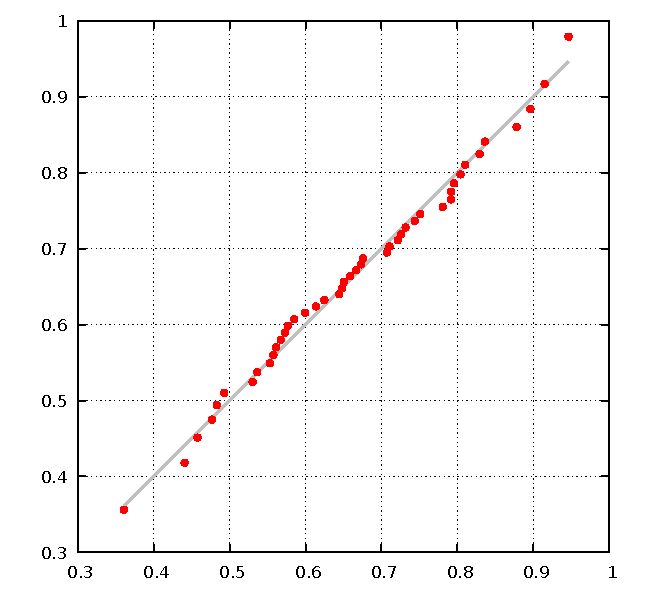
\includegraphics[width=0.3\textwidth]{../PCA/gnuplot/results_qq_diagrams/QQ_diagram12.pdf}}
   \qquad
   \subfloat[Vierter Punkt des Rückens, y-Koordinate]{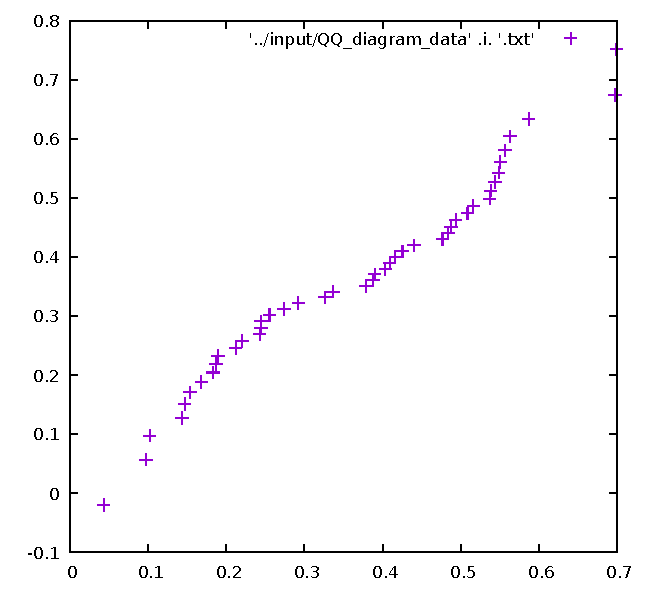
\includegraphics[width=0.3\textwidth]{../PCA/gnuplot/results_qq_diagrams/QQ_diagram13.pdf}}
   \qquad
   \subfloat[Zweiter Punkt des Schwanzes, x-Koordinate]{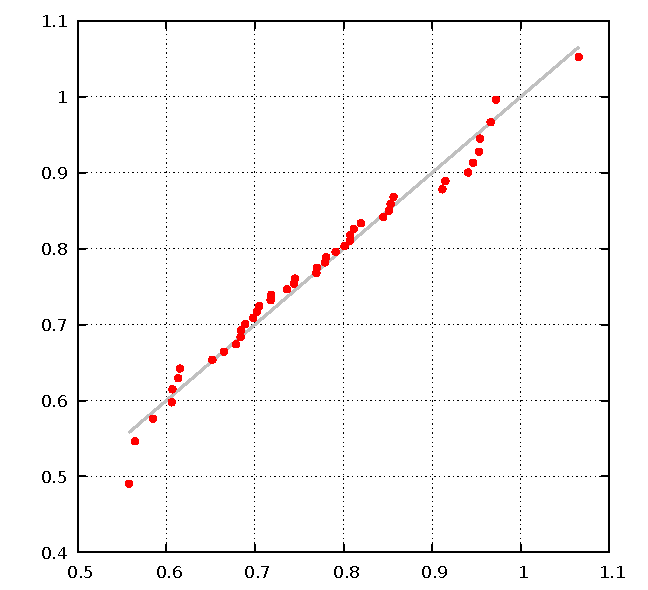
\includegraphics[width=0.3\textwidth]{../PCA/gnuplot/results_qq_diagrams/QQ_diagram14.pdf}}
   \\
   \subfloat[Zweiter Punkt des Schwanzes, y-Koordinate]{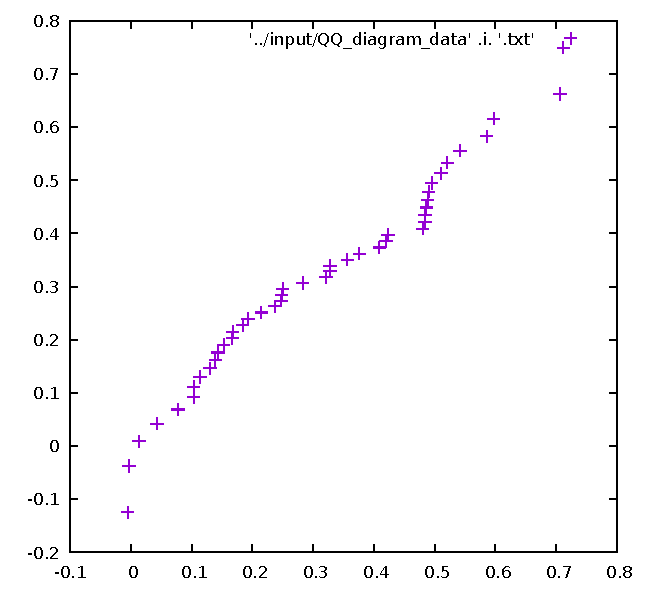
\includegraphics[width=0.3\textwidth]{../PCA/gnuplot/results_qq_diagrams/QQ_diagram15.pdf}}
   \qquad
   \subfloat[Dritter Punkt des Schwanzes, x-Koordinate]{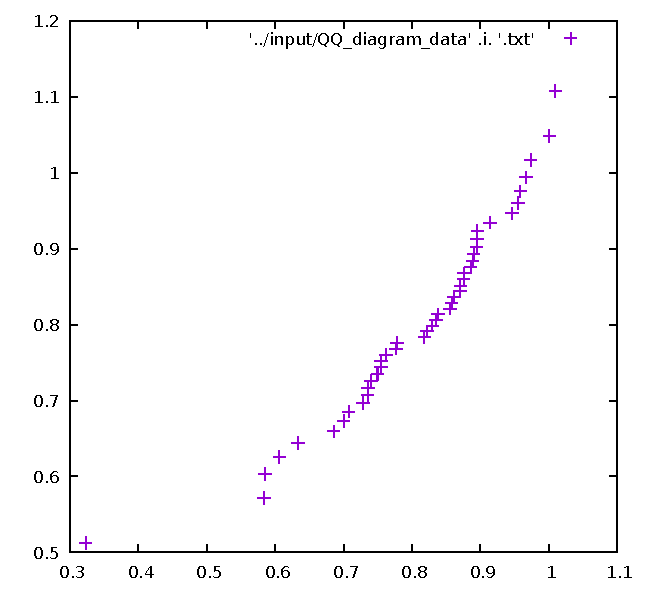
\includegraphics[width=0.3\textwidth]{../PCA/gnuplot/results_qq_diagrams/QQ_diagram16.pdf}}
   \qquad
   \subfloat[Dritter Punkt des Schwanzes, y-Koordinate]{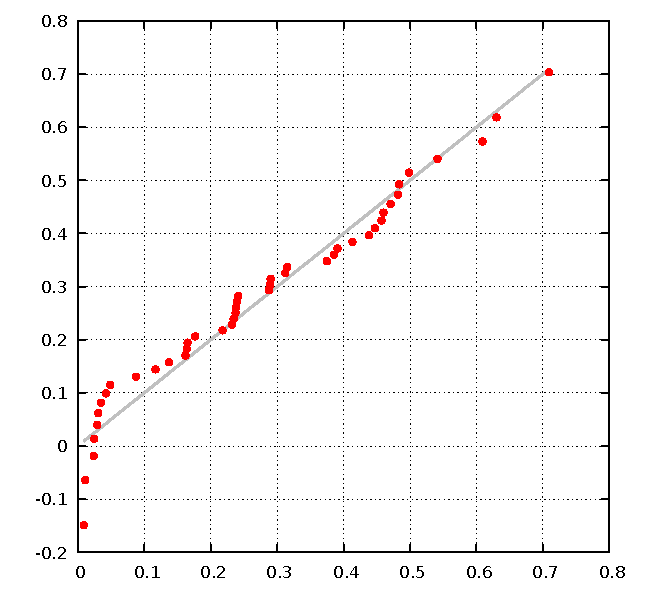
\includegraphics[width=0.3\textwidth]{../PCA/gnuplot/results_qq_diagrams/QQ_diagram17.pdf}}
   \\
   \subfloat[Vierter Punkt des Schwanzes, x-Koordinate]{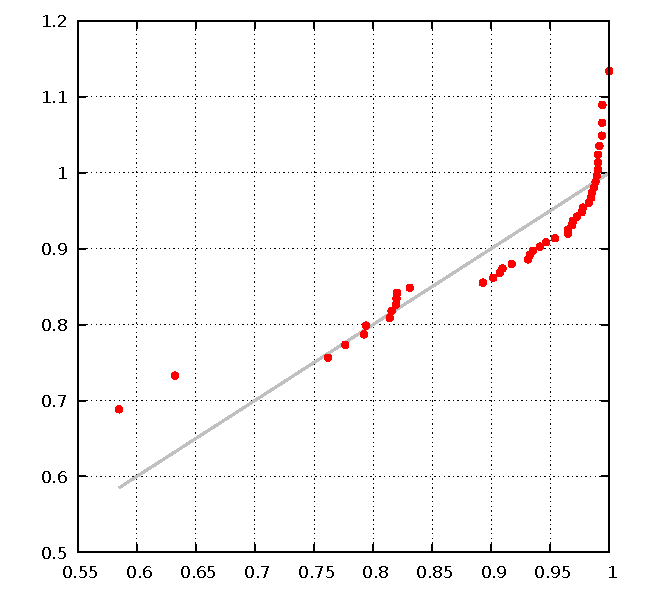
\includegraphics[width=0.3\textwidth]{../PCA/gnuplot/results_qq_diagrams/QQ_diagram18.pdf}}
   \qquad
   \subfloat[Vierter Punkt des Schwanzes, y-Koordinate]{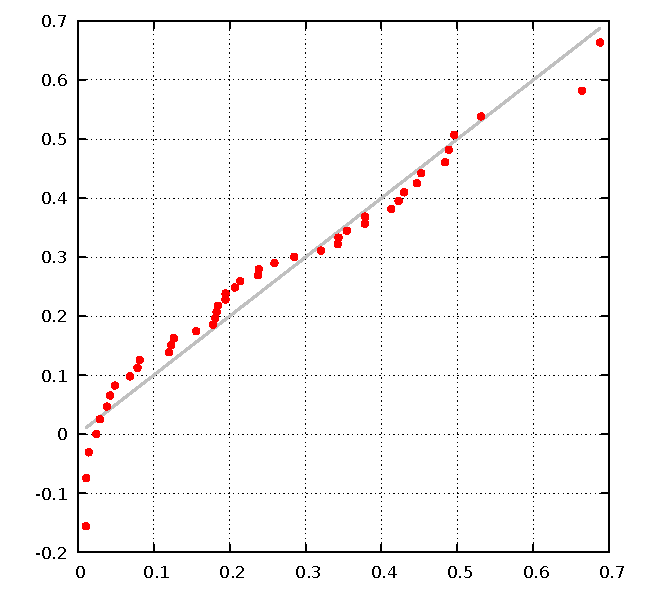
\includegraphics[width=0.3\textwidth]{../PCA/gnuplot/results_qq_diagrams/QQ_diagram19.pdf}}
   
   \caption{Quantil-Quantil-Diagramme für alle Dimensionen der Wirbelsäule}
   \label{qq_diagrams_spine}
  \end{figure}
  \begin{figure}
   \subfloat[Länge Oberarm]{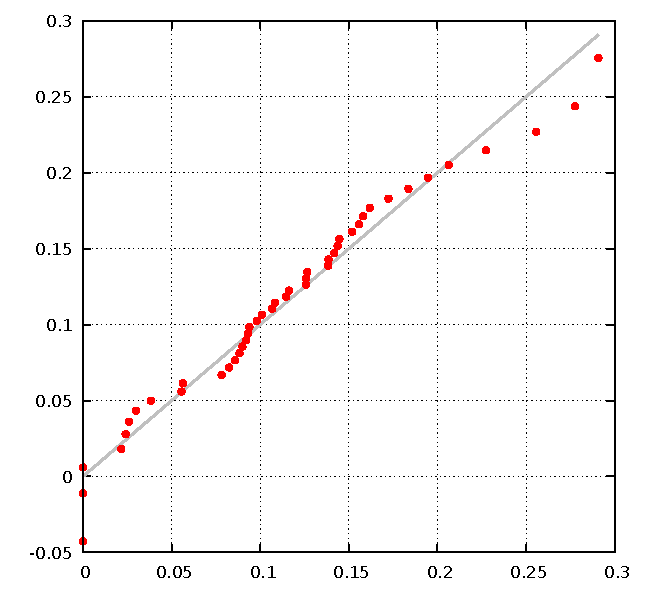
\includegraphics[width=0.3\textwidth]{../PCA/gnuplot/results_qq_diagrams/QQ_diagram22.pdf}}
   \qquad
   \subfloat[Länge Unterarm]{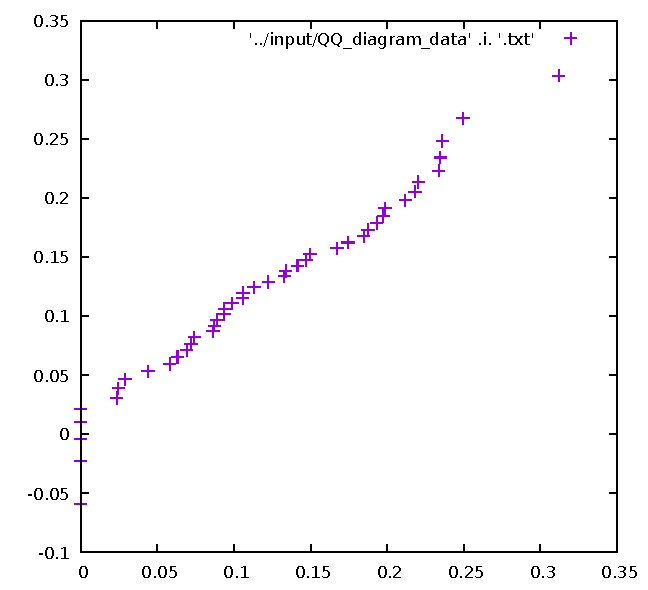
\includegraphics[width=0.3\textwidth]{../PCA/gnuplot/results_qq_diagrams/QQ_diagram23.pdf}}
   \qquad
   \subfloat[Länge Hand]{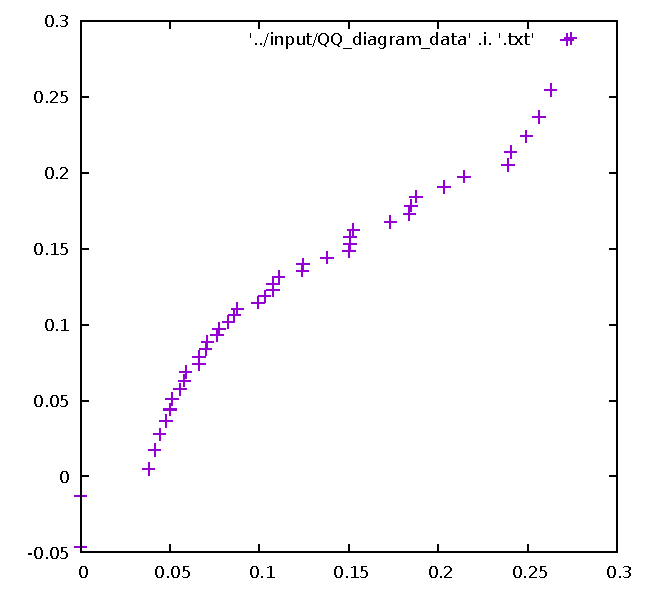
\includegraphics[width=0.3\textwidth]{../PCA/gnuplot/results_qq_diagrams/QQ_diagram24.pdf}}
   \\
   \subfloat[Länge Oberschenkel]{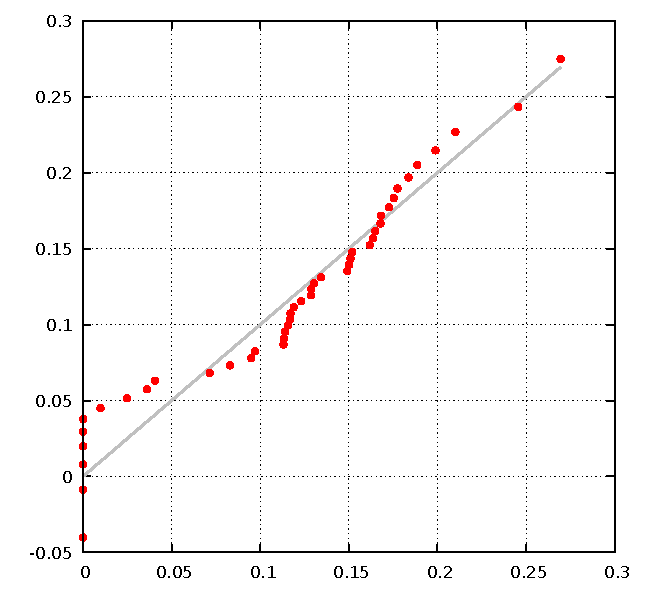
\includegraphics[width=0.3\textwidth]{../PCA/gnuplot/results_qq_diagrams/QQ_diagram25.pdf}}
   \qquad
   \subfloat[Länge Unterschenkel]{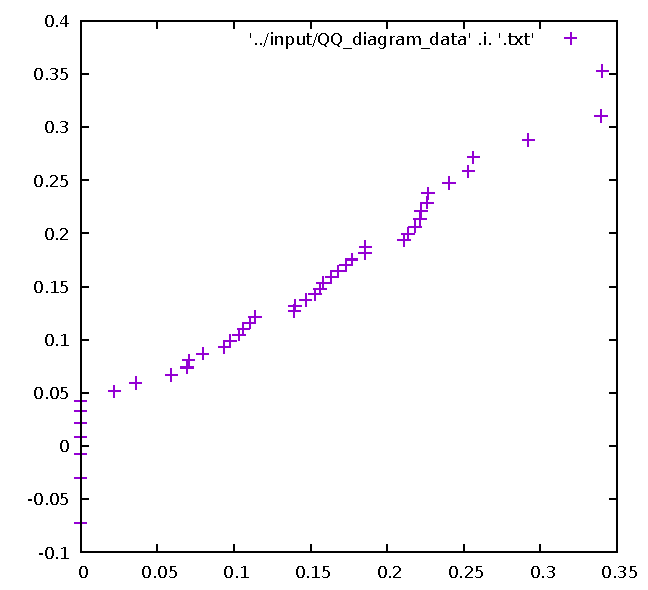
\includegraphics[width=0.3\textwidth]{../PCA/gnuplot/results_qq_diagrams/QQ_diagram26.pdf}}
   \qquad
   \subfloat[Länge Fuß]{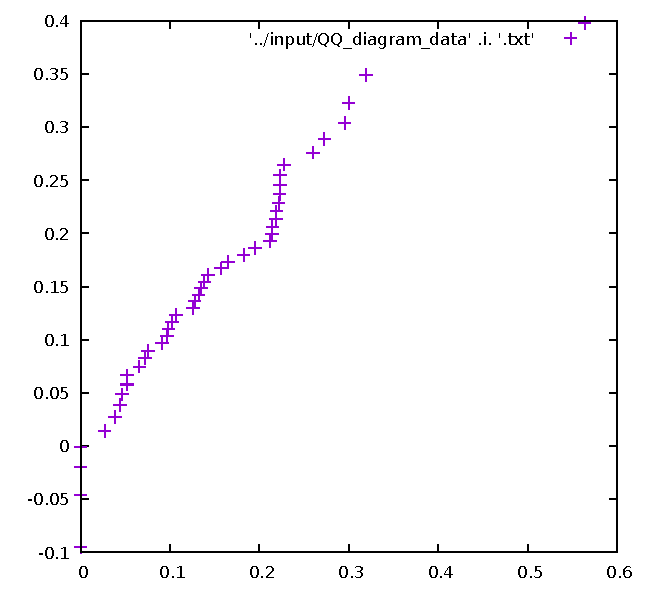
\includegraphics[width=0.3\textwidth]{../PCA/gnuplot/results_qq_diagrams/QQ_diagram27.pdf}}

   \caption{Quantil-Quantil-Diagramme für die Dimensionen der Eingabedaten, die zusätzlich zur Wirbelsäule erhoben wurden. Nicht dargestellt ist das binäre Attribut \emph{Flügel} und die Anzahl der Beine mit Bodenkontakt.}
   \label{qq_diagrams_rest}
  \end{figure}
  
  
 %-------------------------------------
 \section{Mit PCA erzeugte Datenpunkte}
 
 
 \begin{figure}
   \centering
   \subfloat[1-, \emph{Flügel} $0,38$, \emph{Beine} $1,6$, \emph{Gewicht} $92$kg]{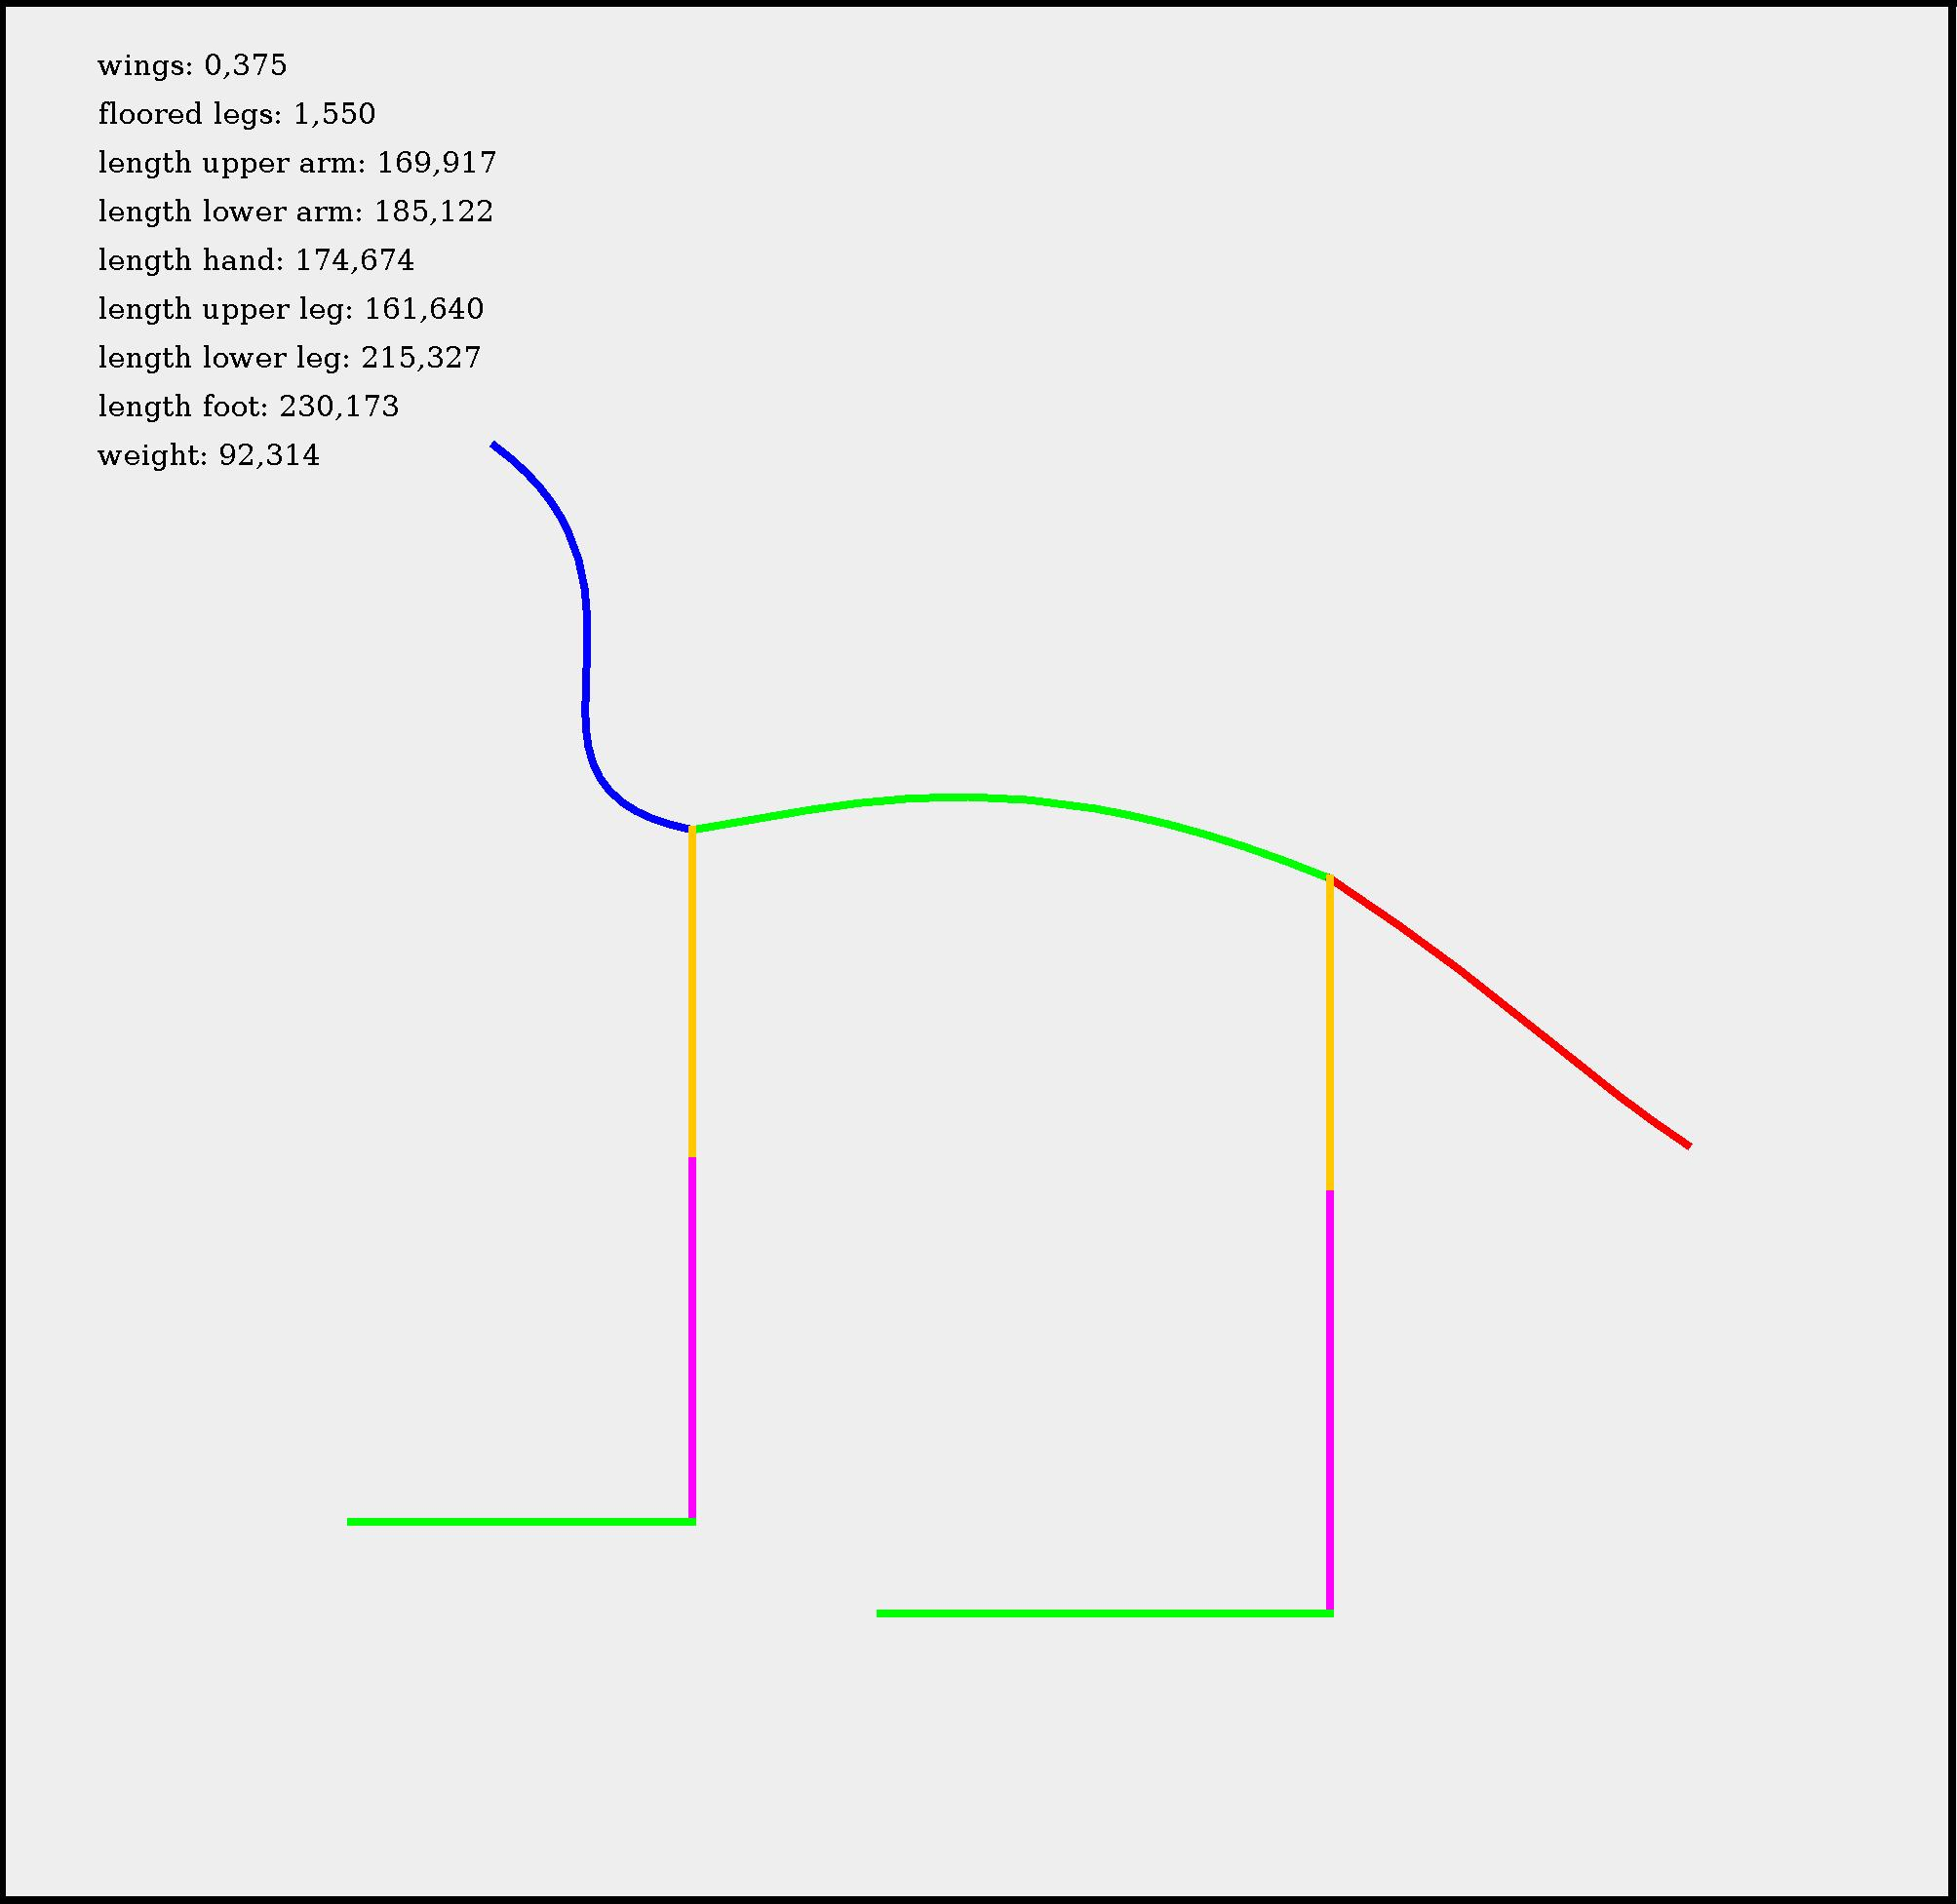
\includegraphics[width=0.45\textwidth]{../PCA/sqrtEV_log_weight_downscaled_wings_legs_and_weight/EV1_neg.jpg}}
   \qquad
   \subfloat[1+, \emph{Flügel} $-0,057$, \emph{Beine} $1,2$, \emph{Gewicht} $94$kg]{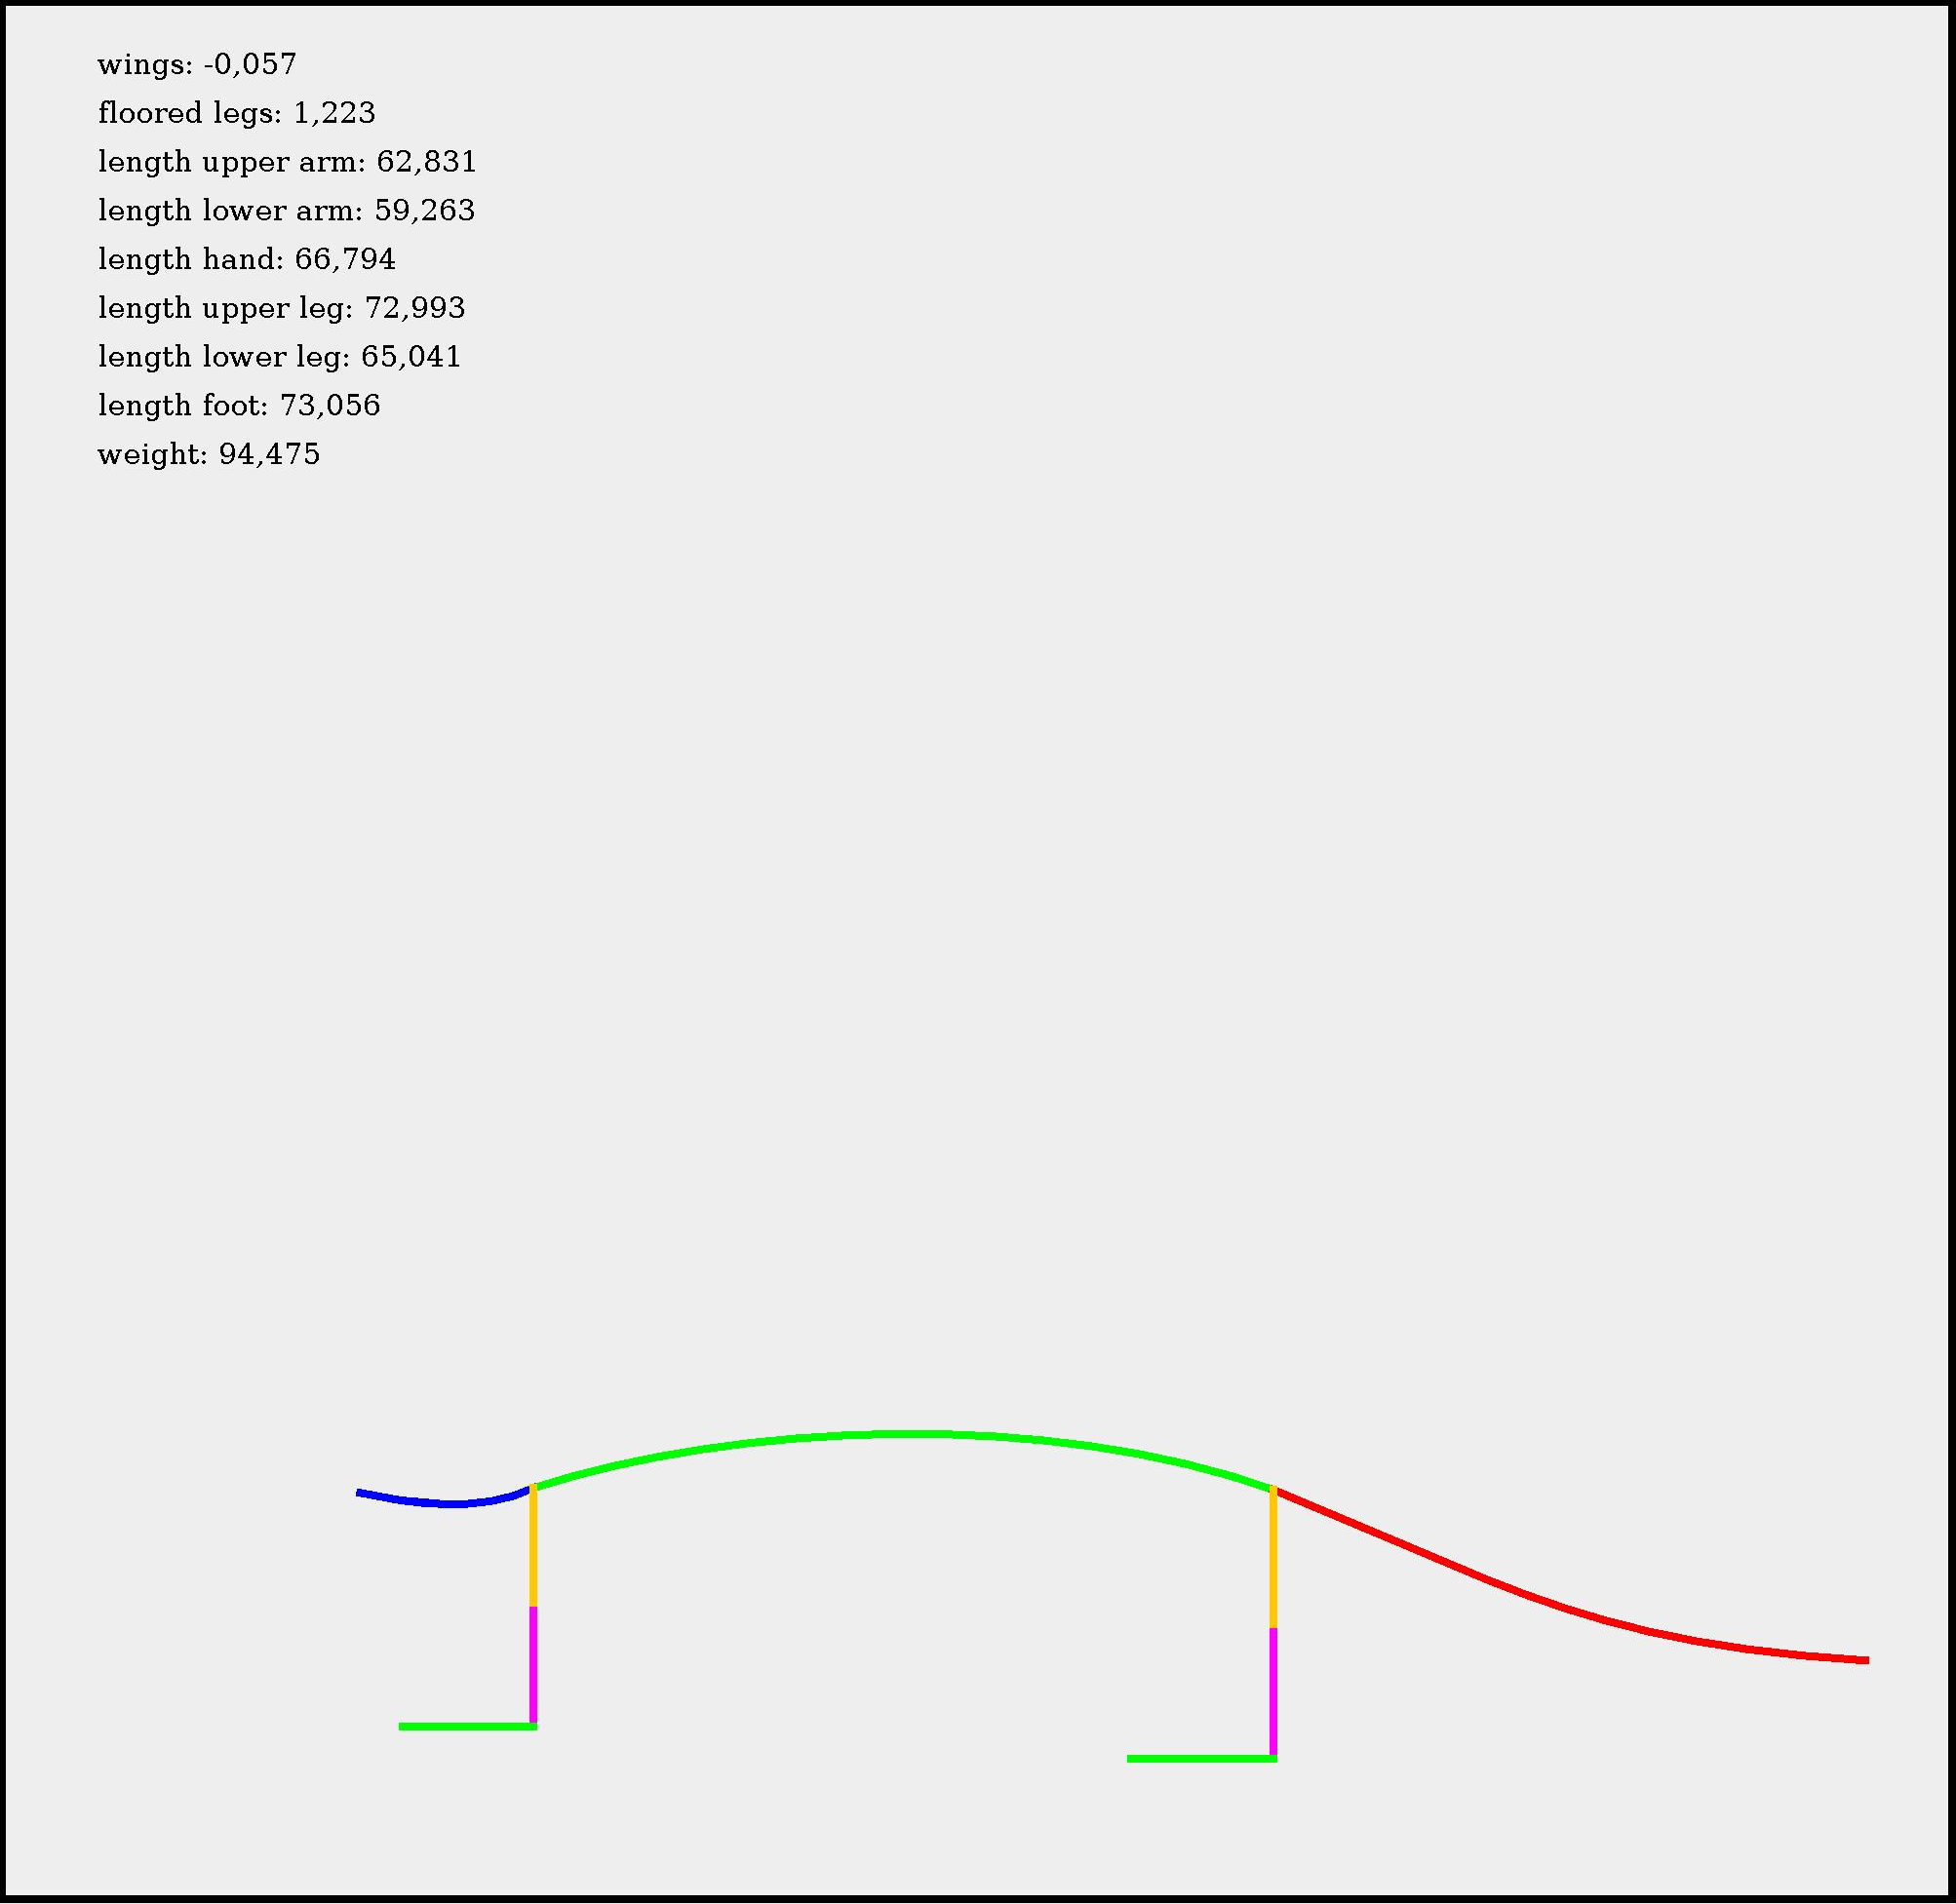
\includegraphics[width=0.45\textwidth]{../PCA/sqrtEV_log_weight_downscaled_wings_legs_and_weight/EV1_pos.jpg}}
   \\
   \subfloat[2-, \emph{Flügel} $0,014$, \emph{Beine} $1,4$, \emph{Gewicht} $94$kg]{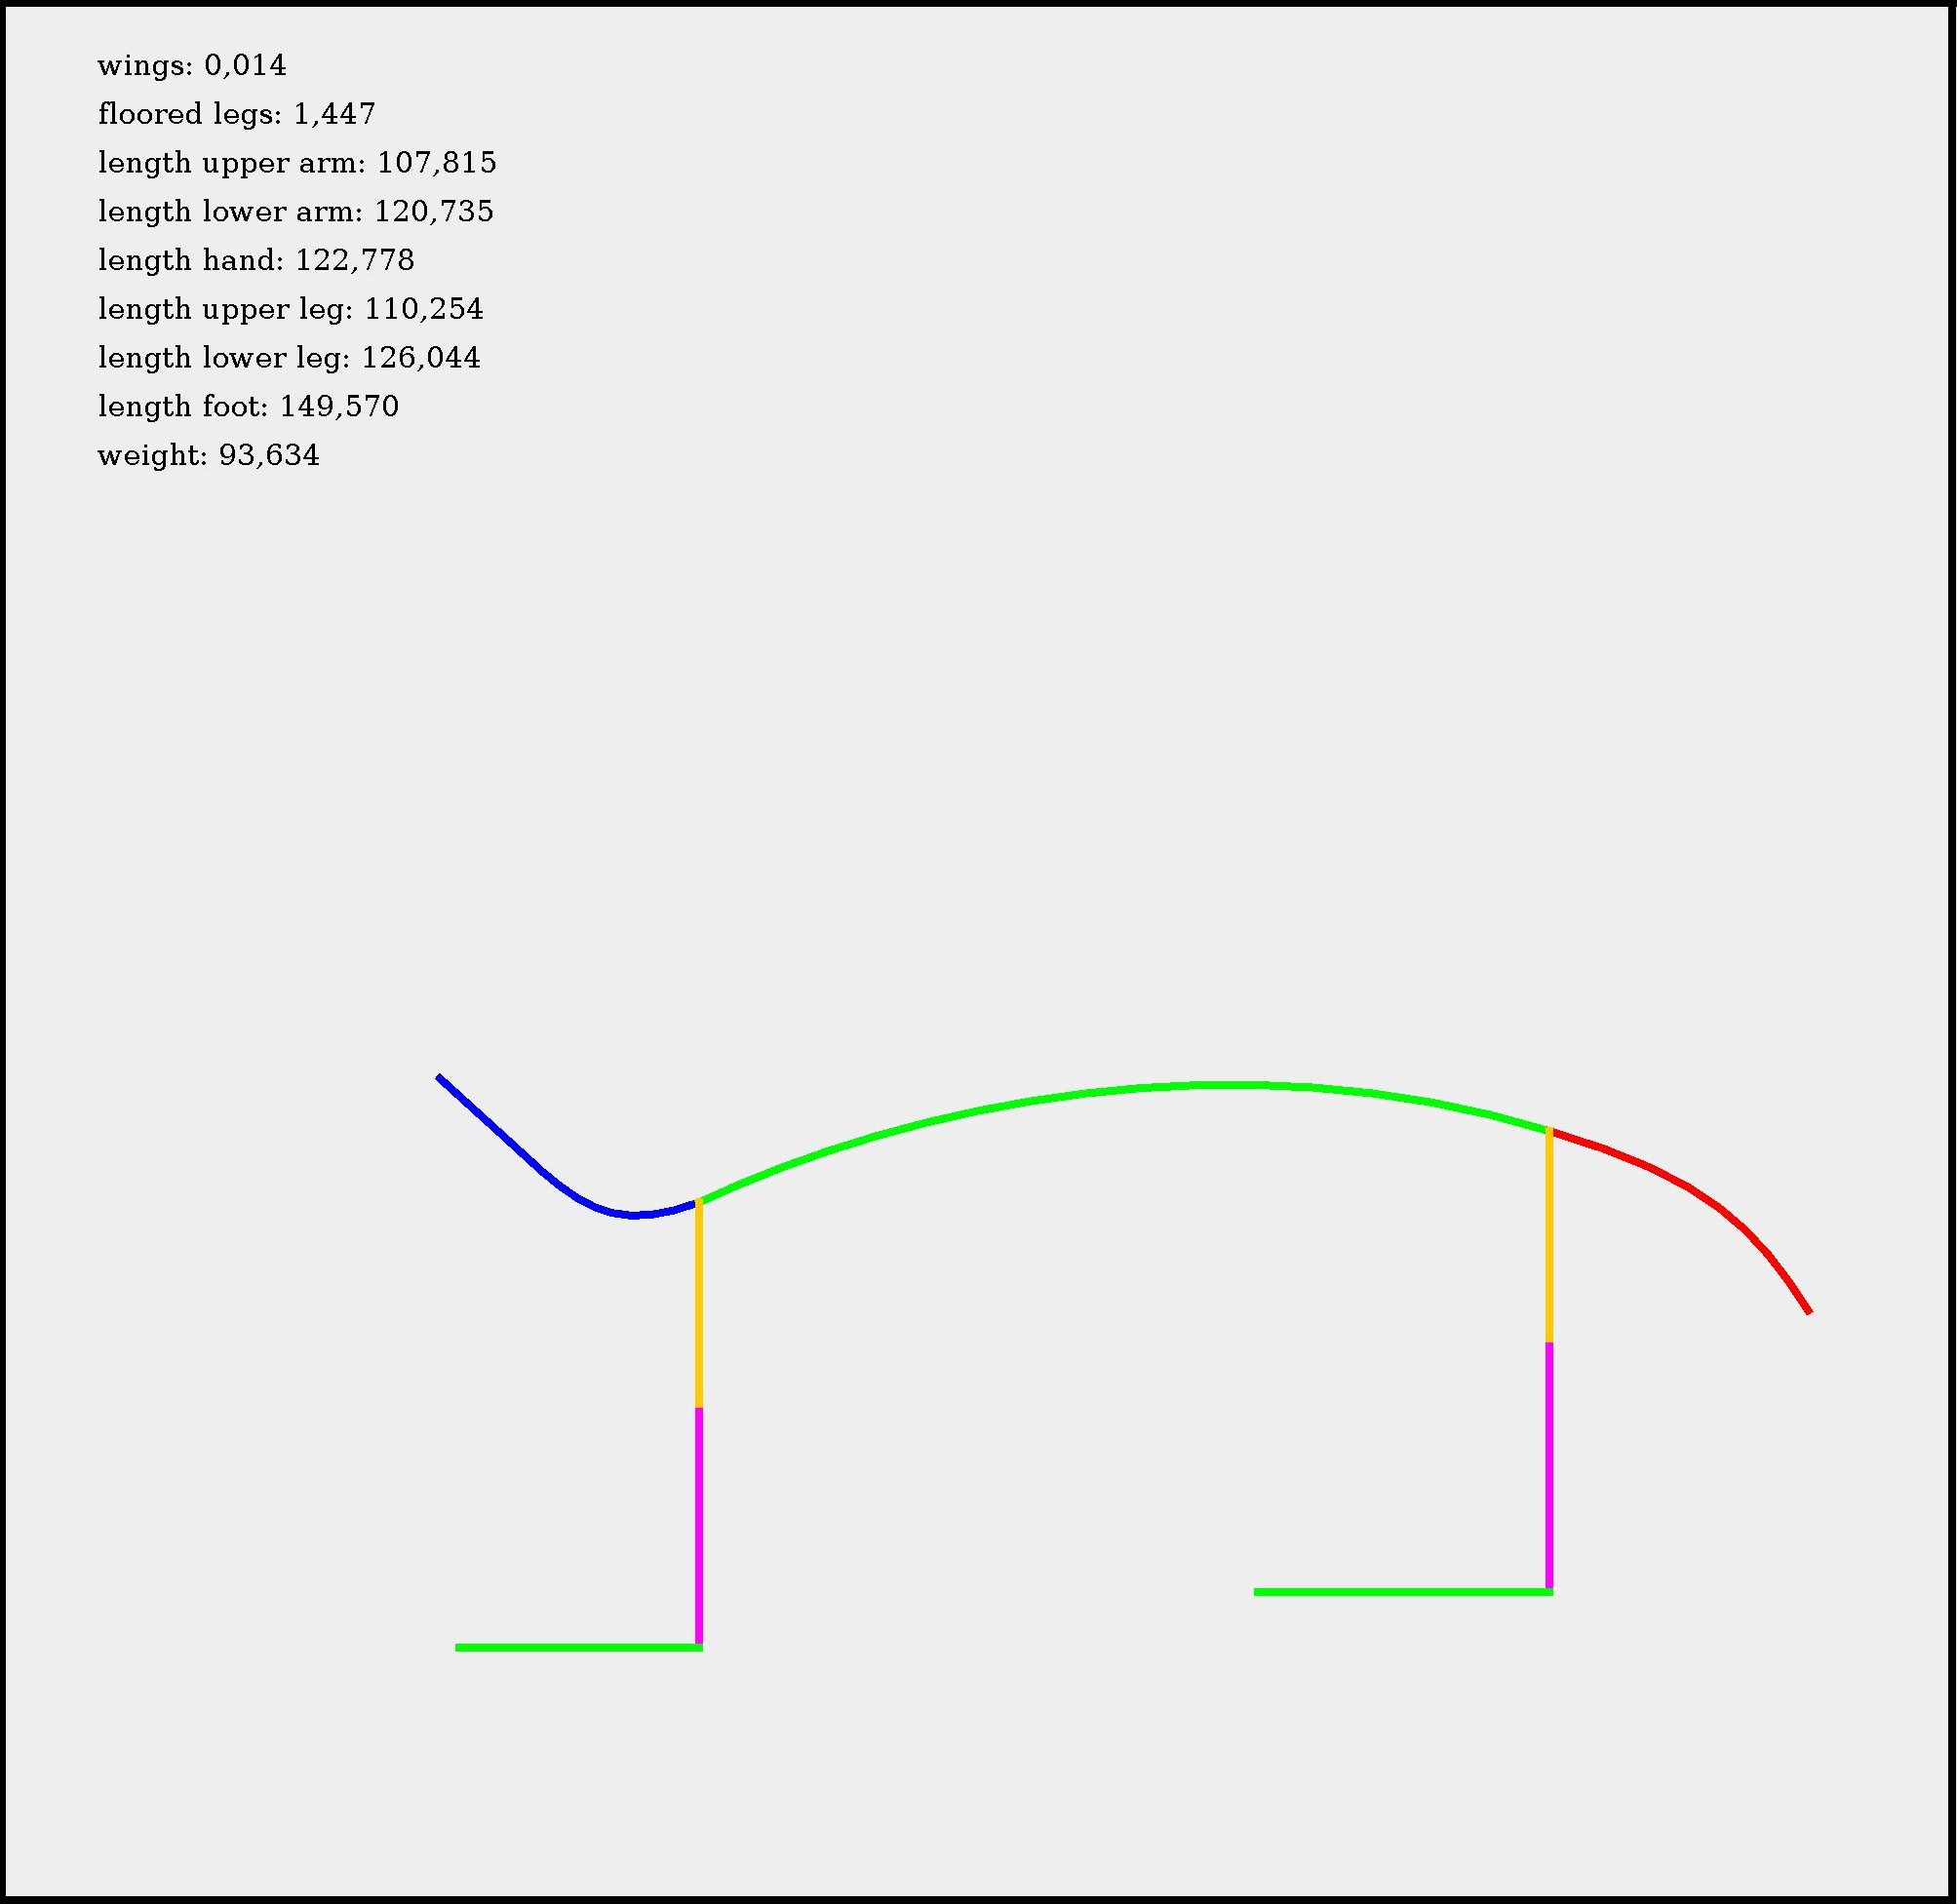
\includegraphics[width=0.45\textwidth]{../PCA/sqrtEV_log_weight_downscaled_wings_legs_and_weight/EV2_neg.jpg}}
   \qquad
   \subfloat[2+, \emph{Flügel} $0,3$, \emph{Beine} $1,3$, \emph{Gewicht} $93$kg]{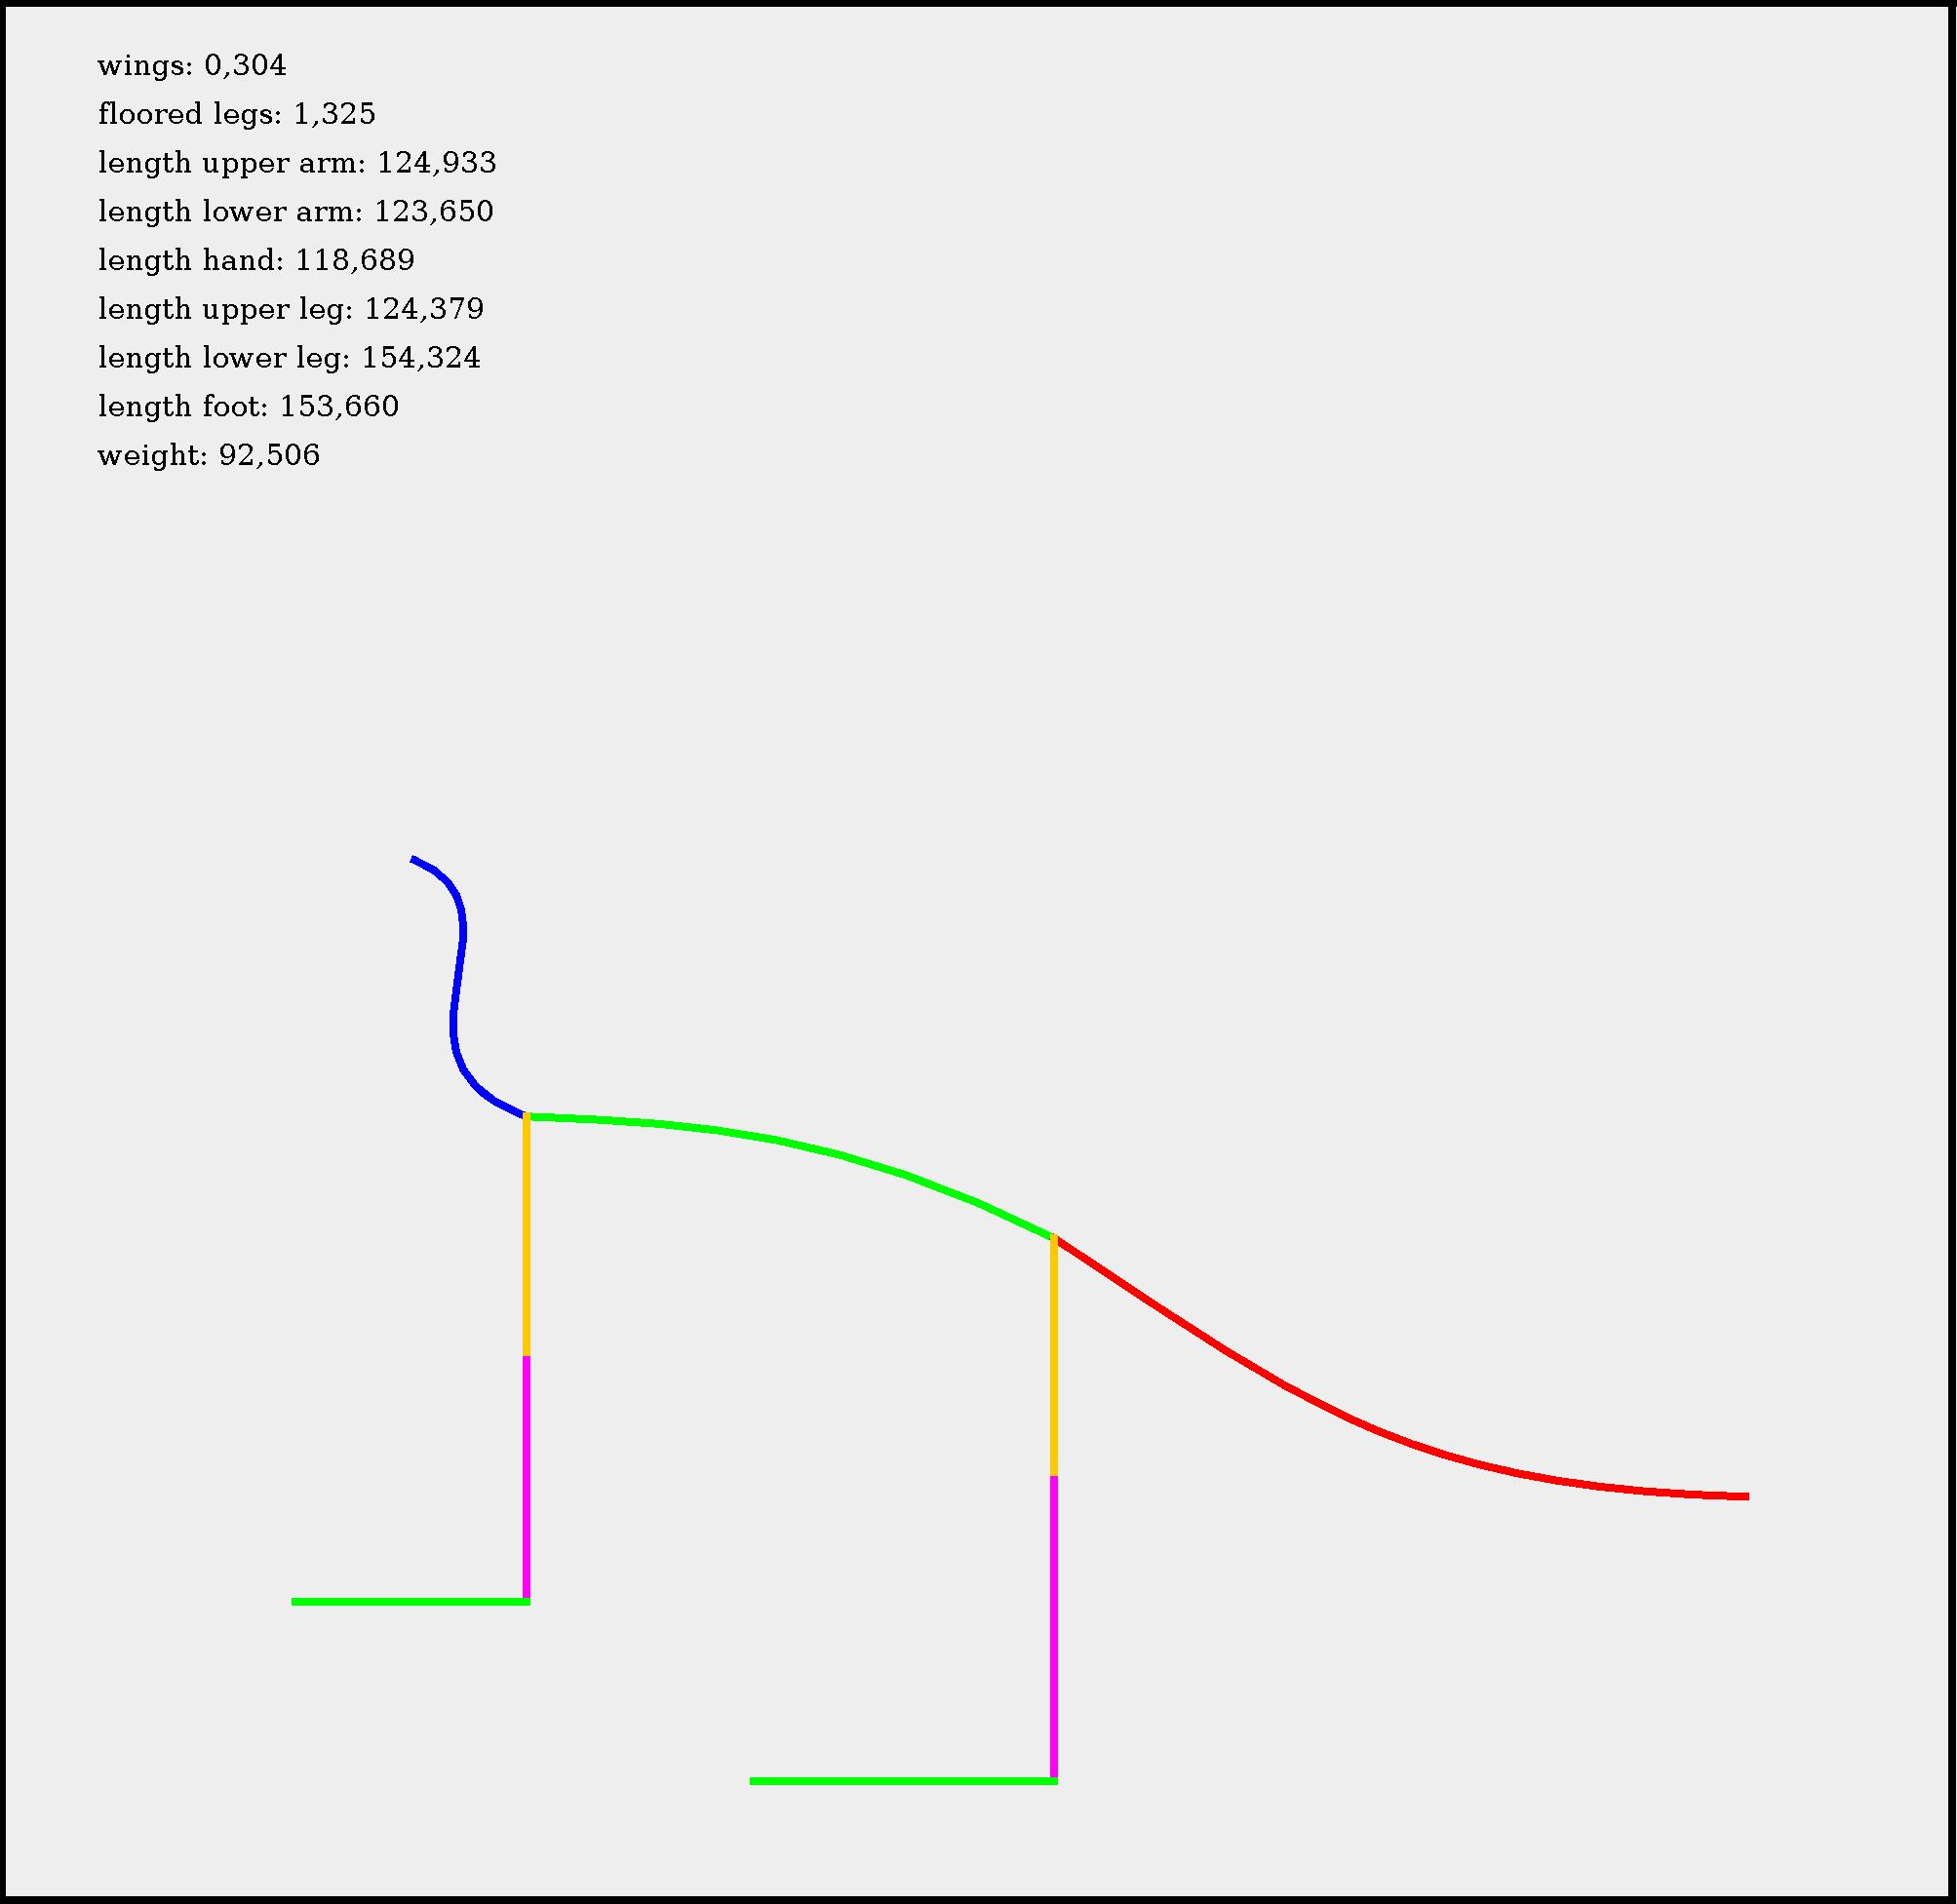
\includegraphics[width=0.45\textwidth]{../PCA/sqrtEV_log_weight_downscaled_wings_legs_and_weight/EV2_pos.jpg}}
   \\
   \subfloat[3-, \emph{Flügel} $0,11$, \emph{Beine} $1,6$, \emph{Gewicht} $93$kg]{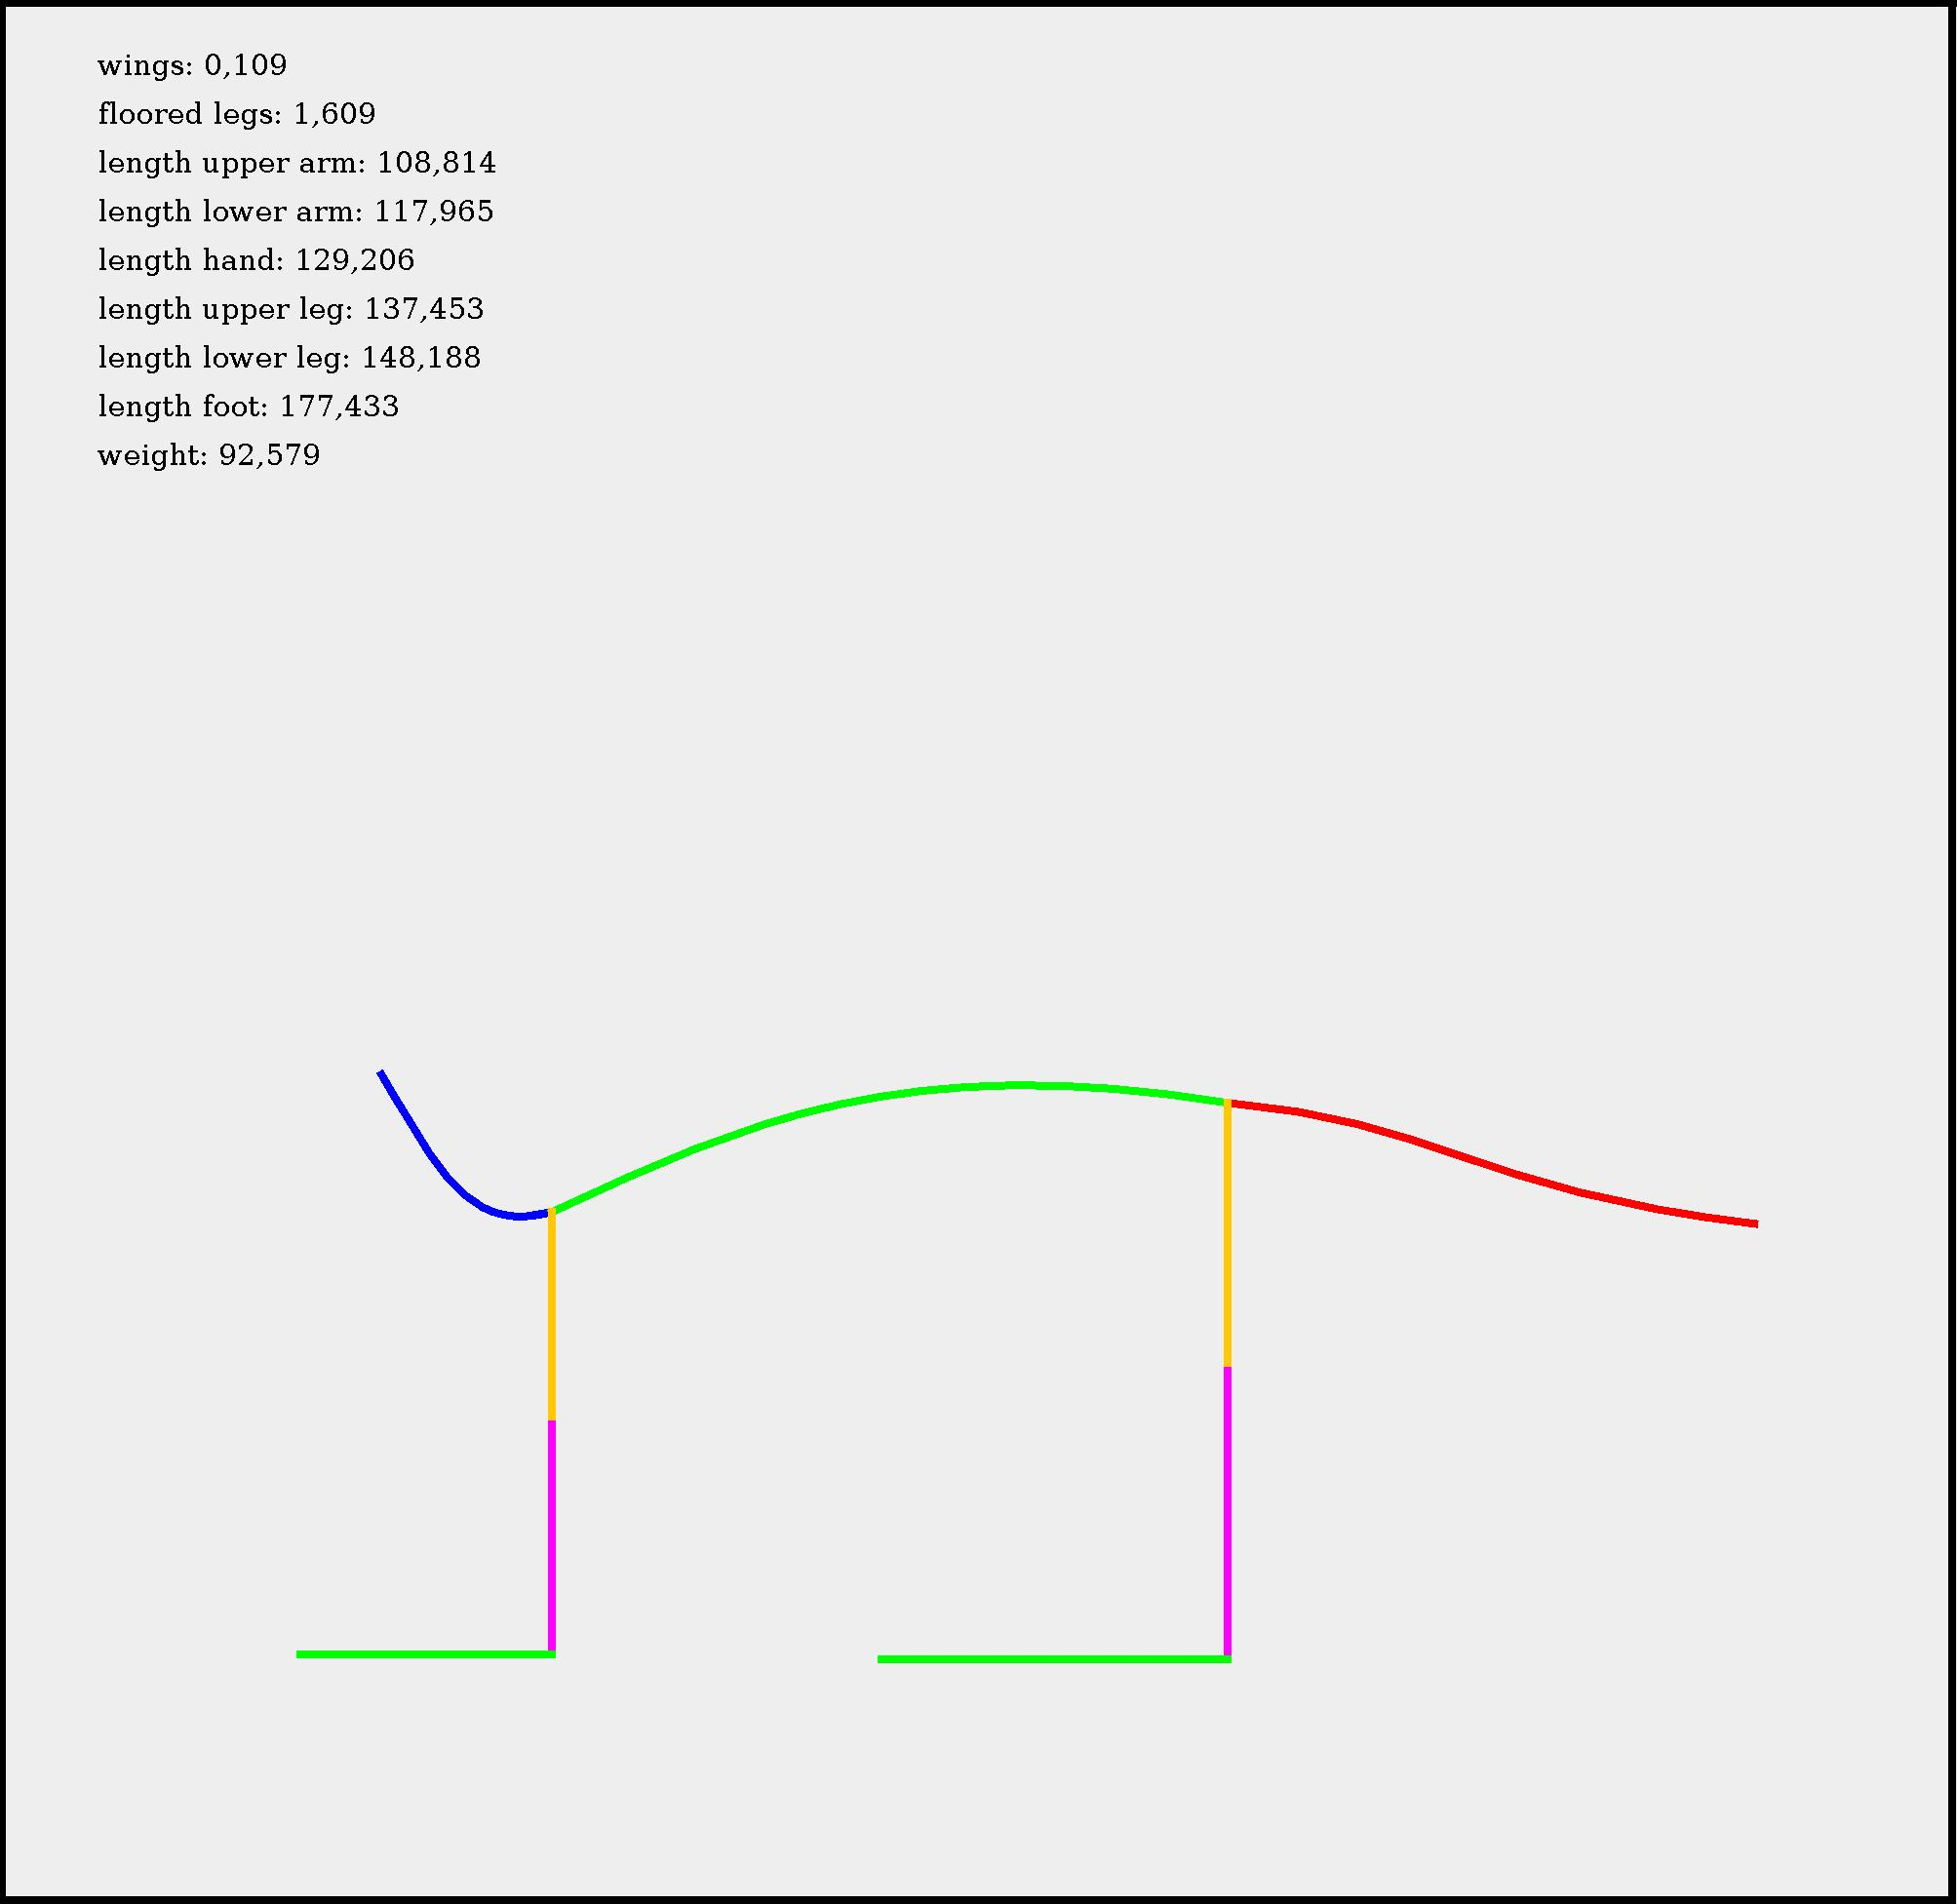
\includegraphics[width=0.45\textwidth]{../PCA/sqrtEV_log_weight_downscaled_wings_legs_and_weight/EV3_neg.jpg}}
   \qquad
   \subfloat[3+, \emph{Flügel} $0,21$, \emph{Beine} $1,2$, \emph{Gewicht} $93$kg]{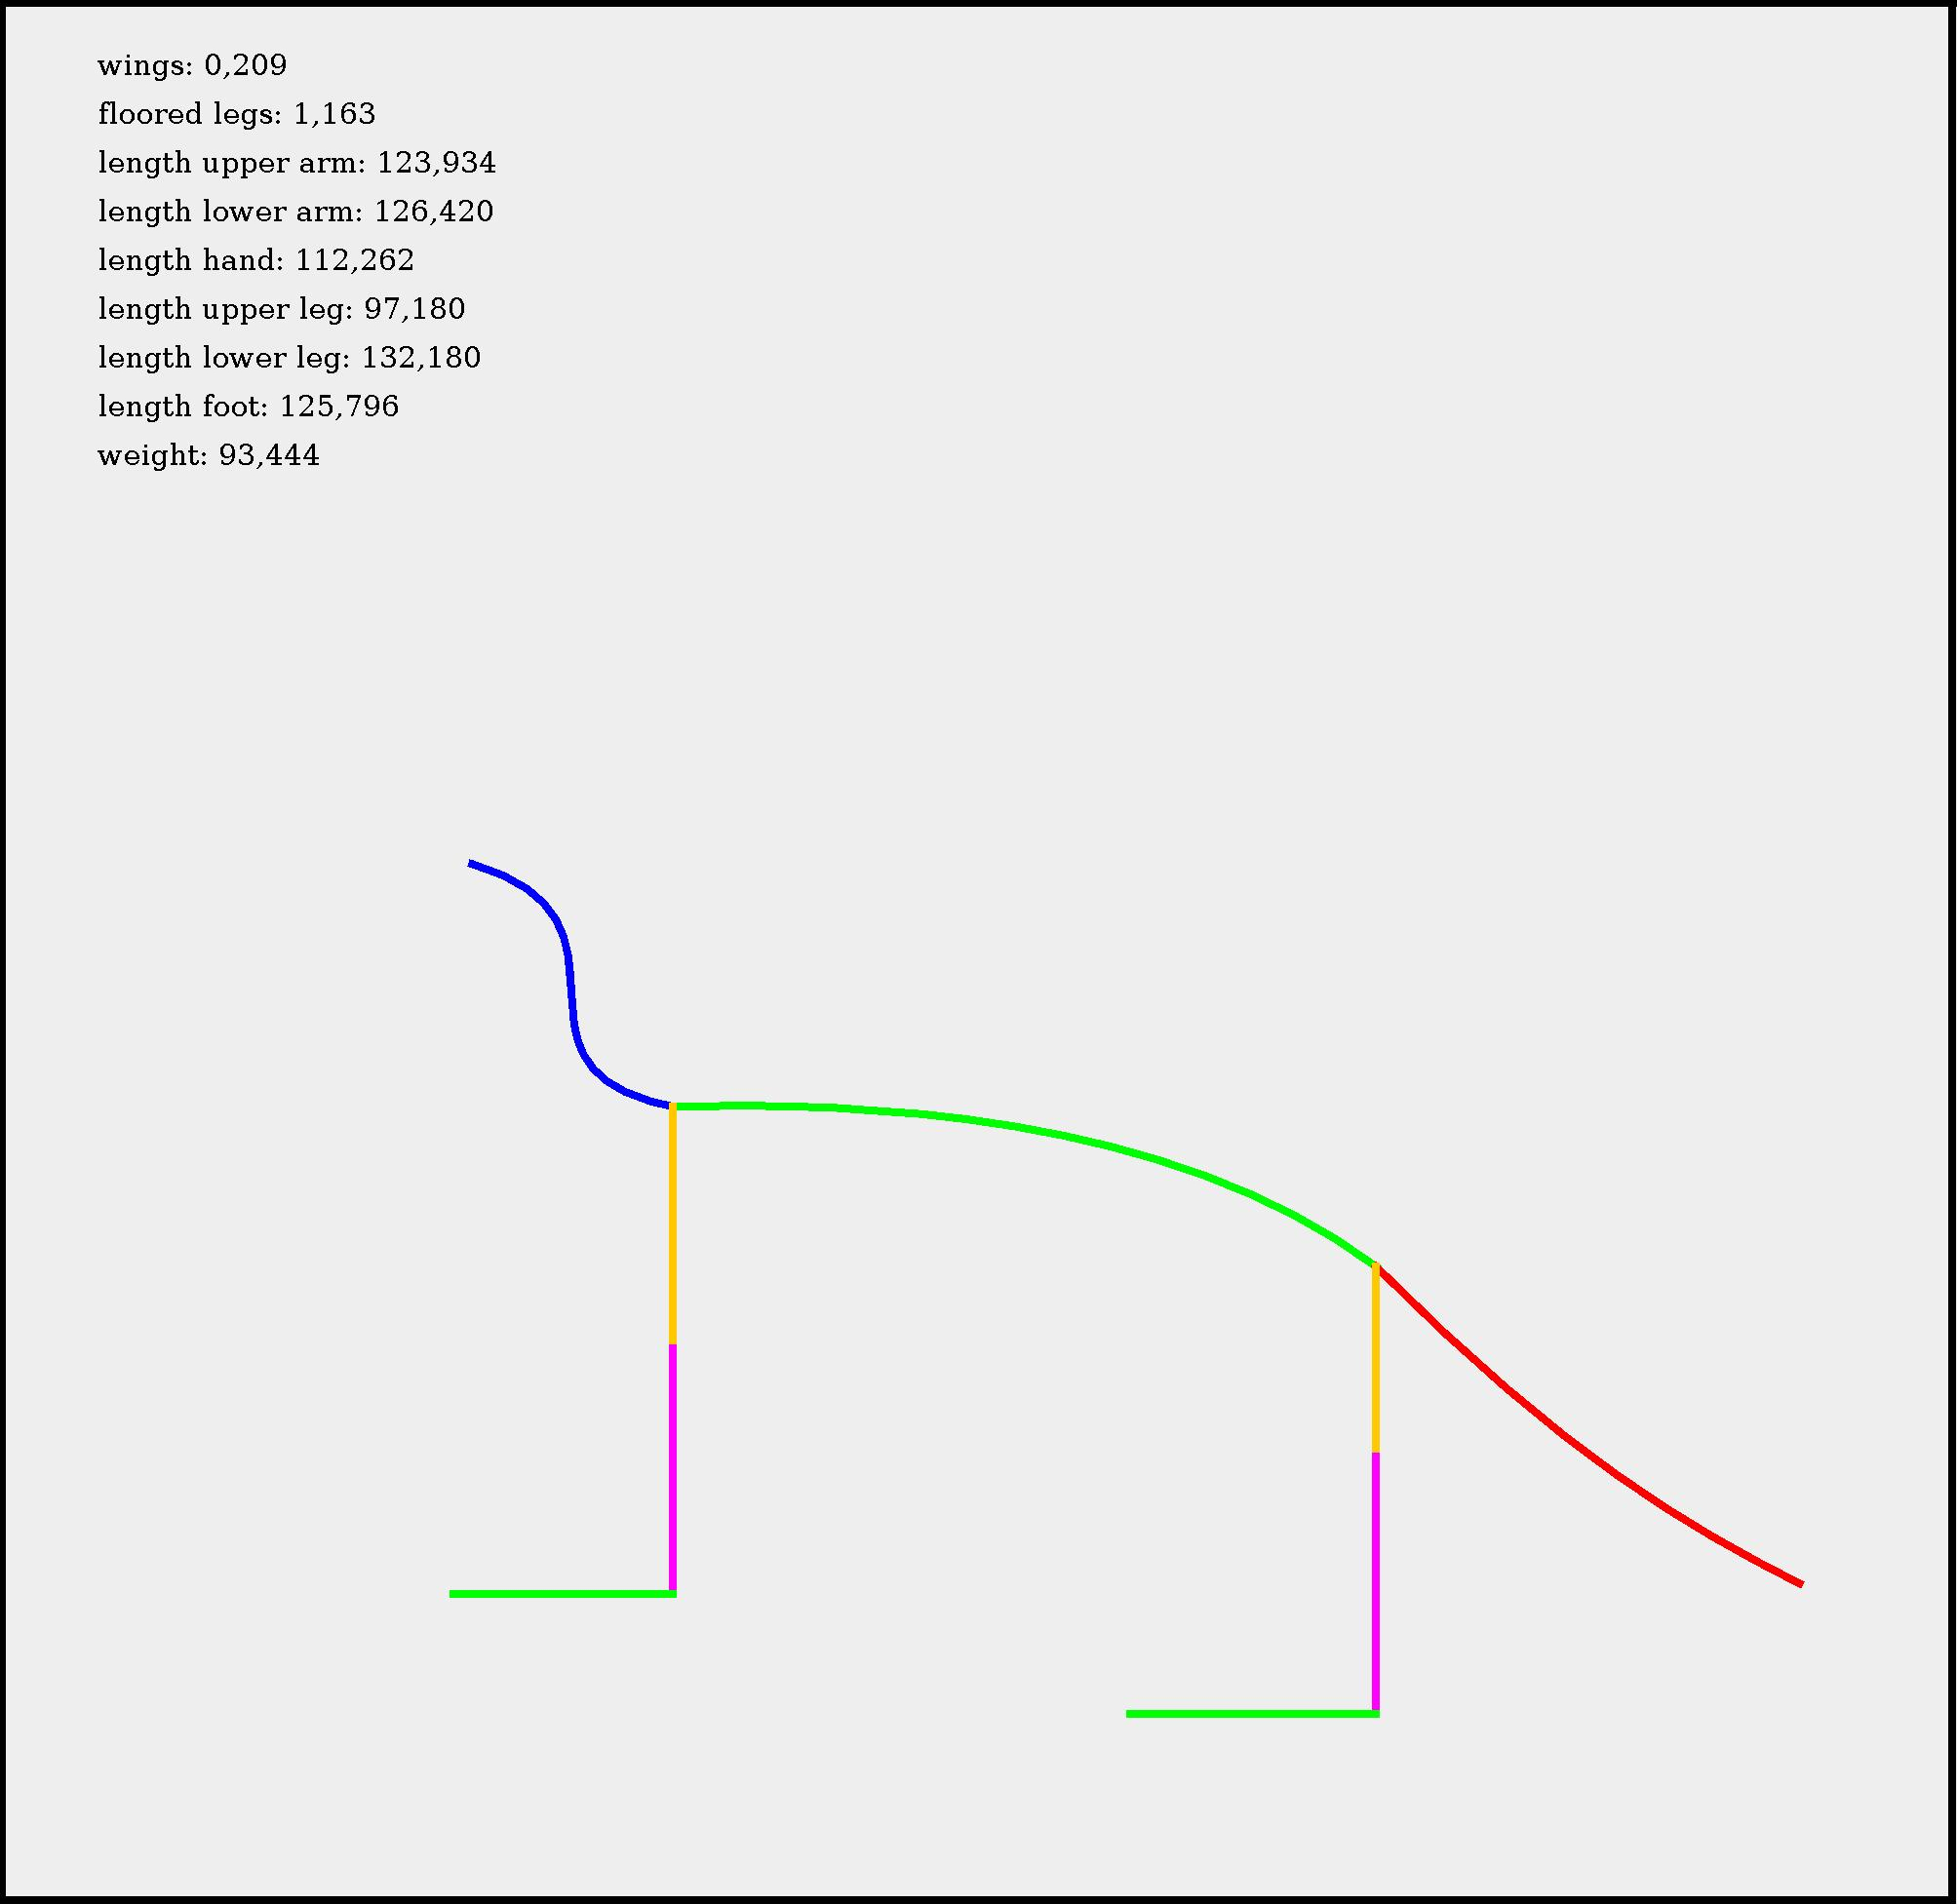
\includegraphics[width=0.45\textwidth]{../PCA/sqrtEV_log_weight_downscaled_wings_legs_and_weight/EV3_pos.jpg}}
   \phantomcaption
 \end{figure}
 \begin{figure}
   \ContinuedFloat
   \centering
   \subfloat[4-, \emph{Flügel} $0,3$, \emph{Beine} $1$, \emph{Gewicht} $92$kg]{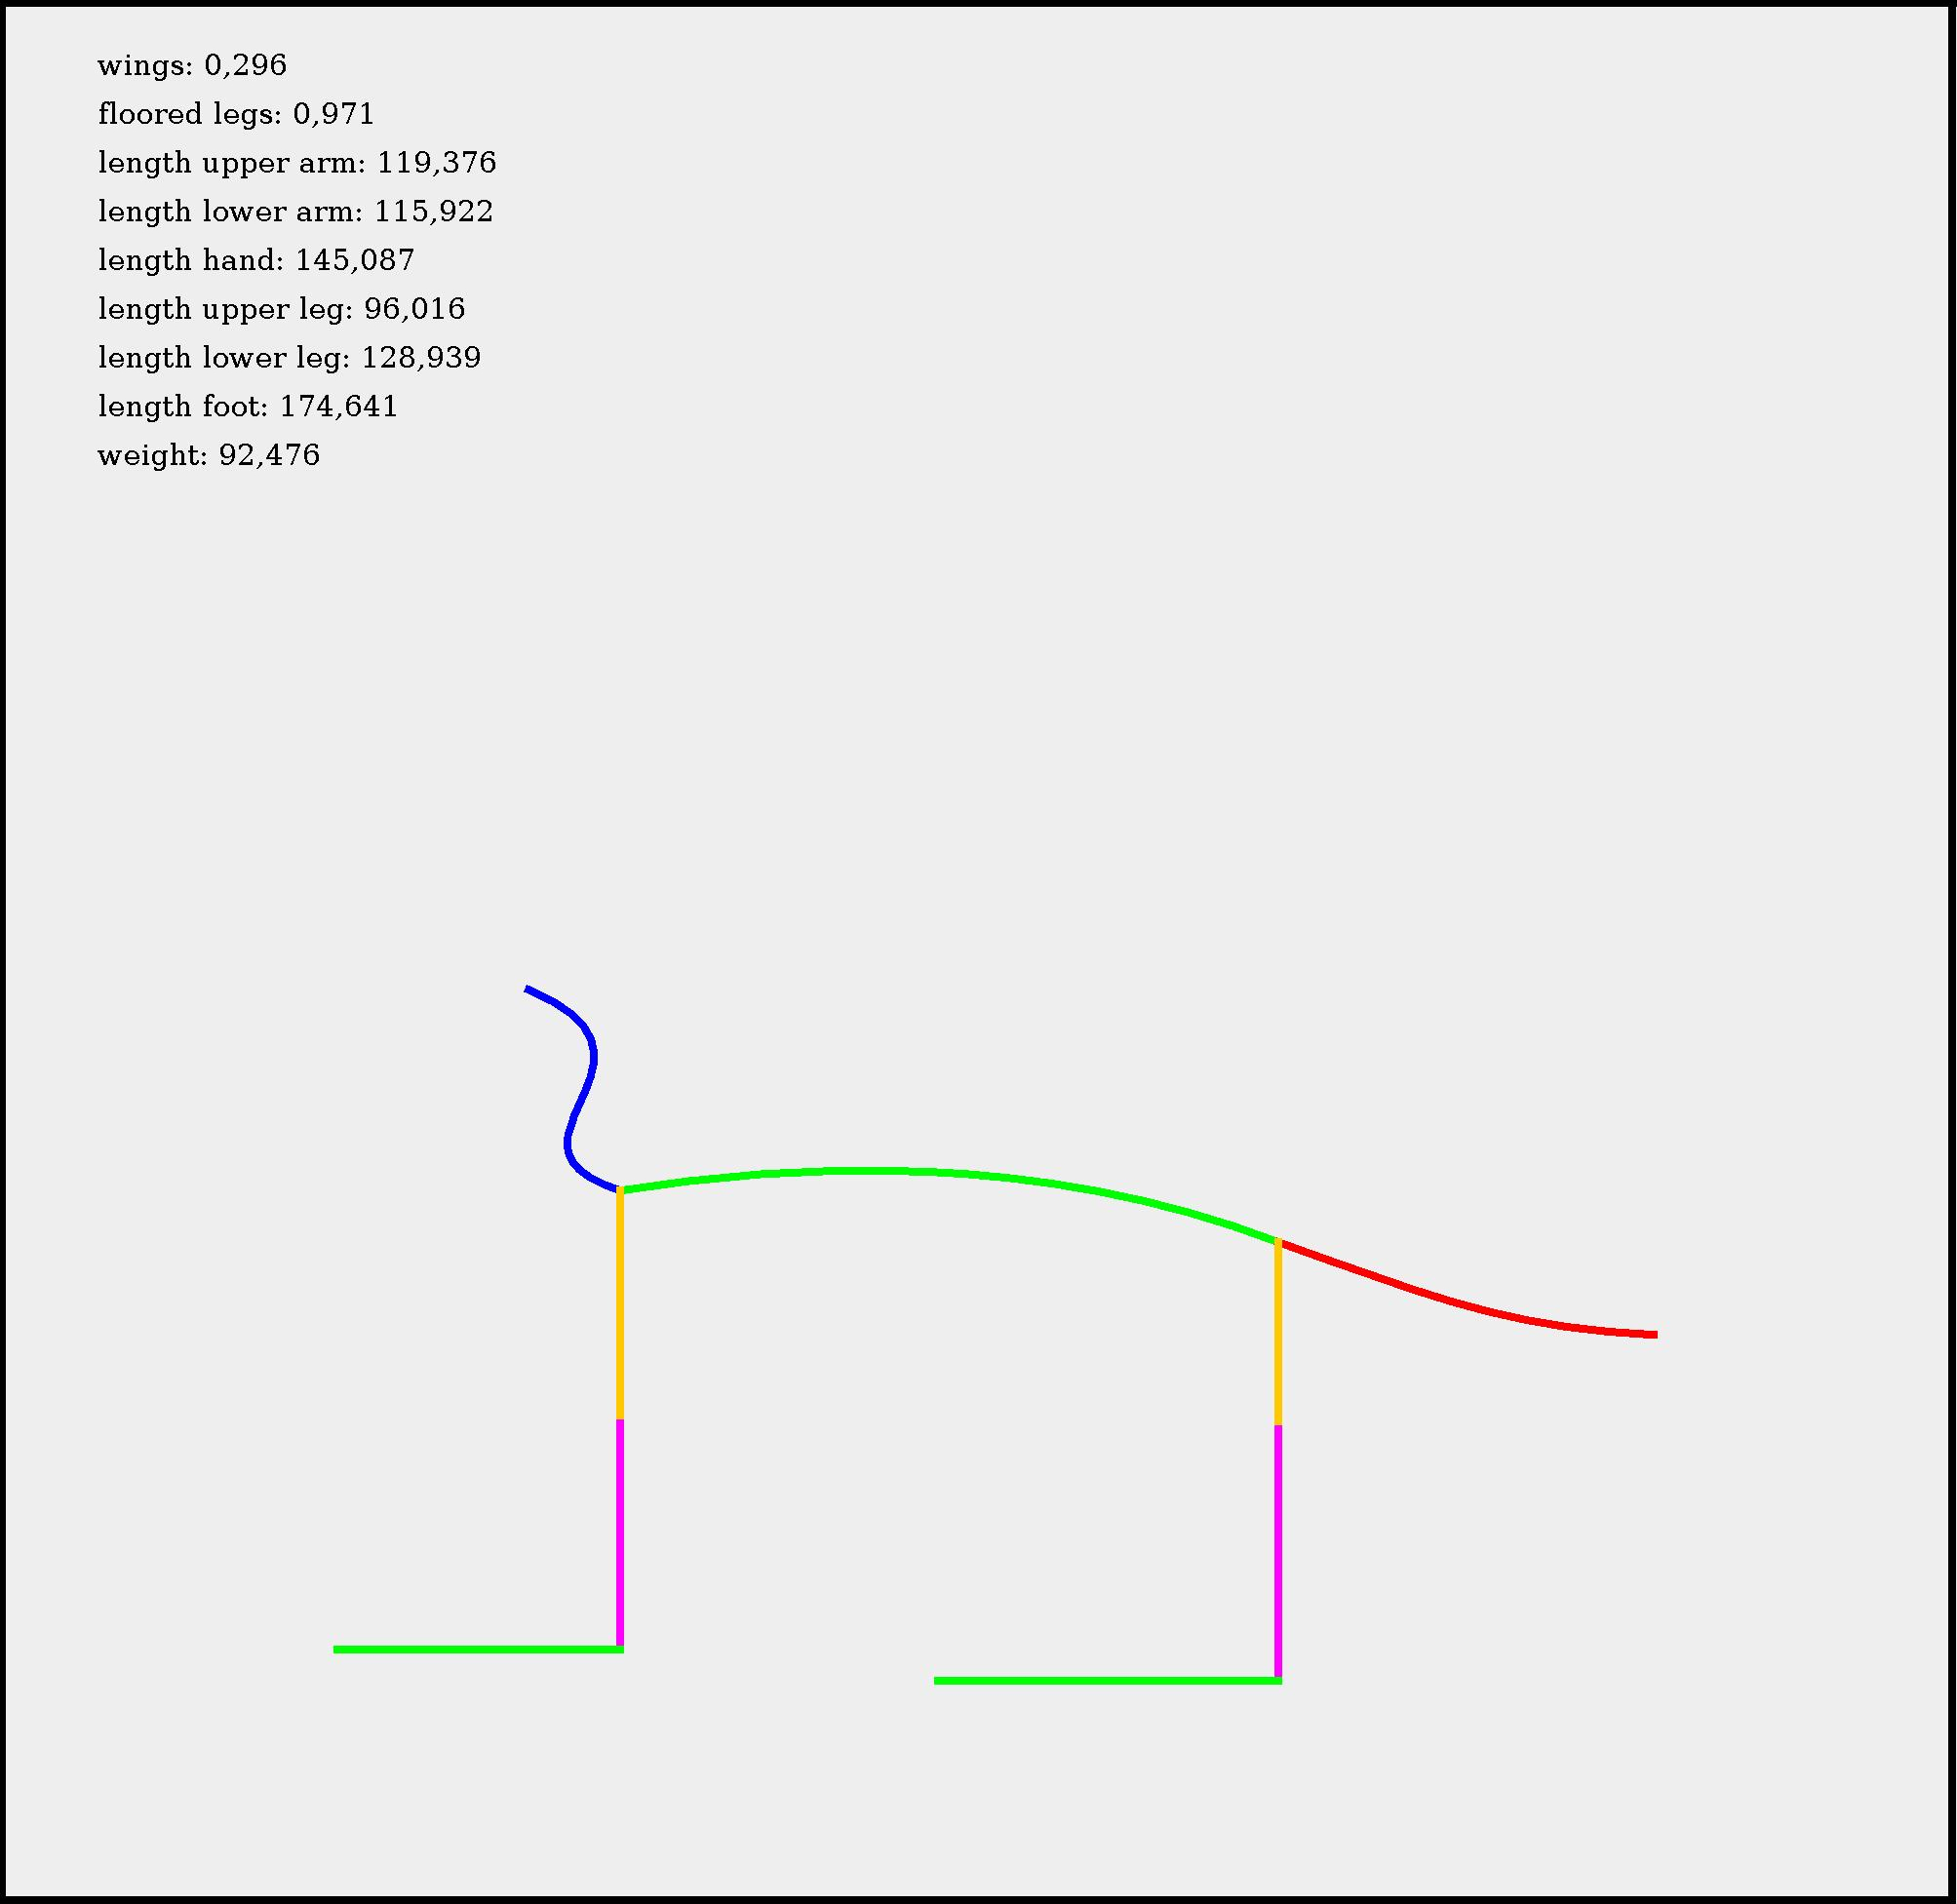
\includegraphics[width=0.45\textwidth]{../PCA/sqrtEV_log_weight_downscaled_wings_legs_and_weight/EV4_neg.jpg}}
   \qquad
   \subfloat[4+, \emph{Flügel} $0,022$, \emph{Beine} $1,8$, \emph{Gewicht} $94$kg]{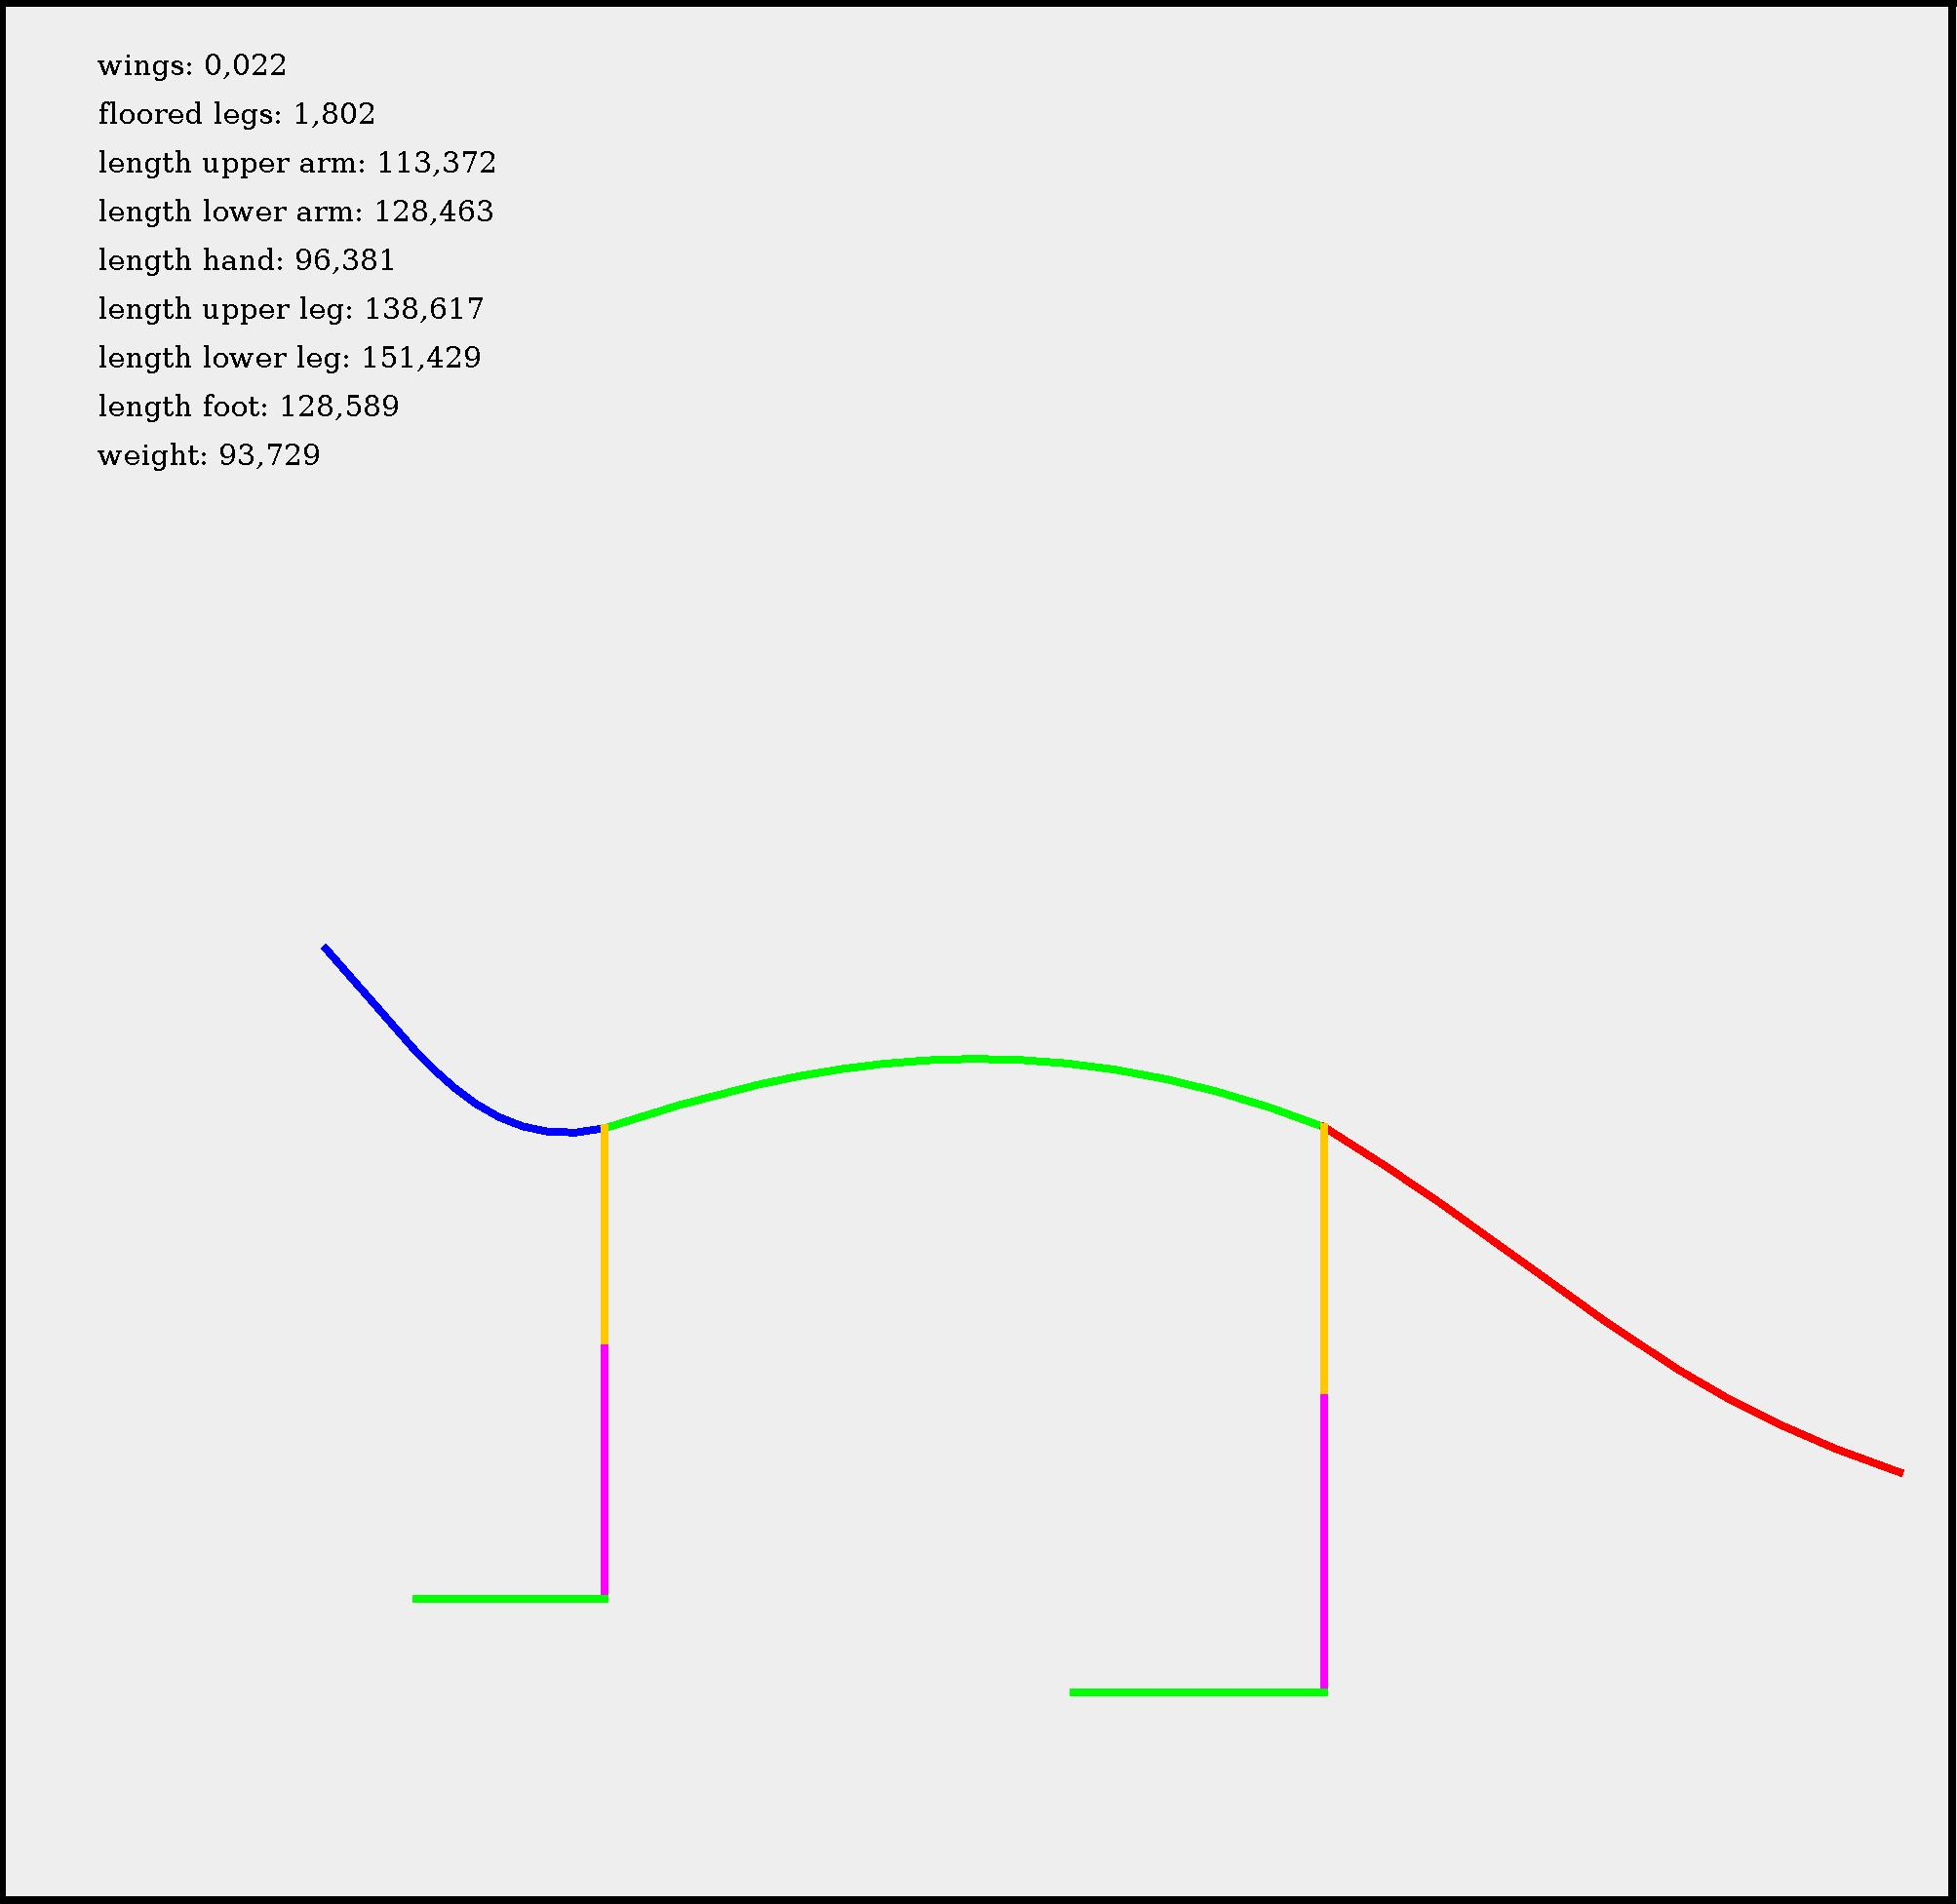
\includegraphics[width=0.45\textwidth]{../PCA/sqrtEV_log_weight_downscaled_wings_legs_and_weight/EV4_pos.jpg}}
   \\
   \subfloat[5-, \emph{Flügel} $0,08$, \emph{Beine} $1,6$, \emph{Gewicht} $93$kg]{\includegraphics[width=0.45\textwidth]{../PCA/sqrtEV_log_weight_downscaled_wings_legs_and_weight/EV5_neg.jpg}}
   \qquad
   \subfloat[5+, \emph{Flügel} $0,24$, \emph{Beine} $1,2$, \emph{Gewicht} $93$kg]{\includegraphics[width=0.45\textwidth]{../PCA/sqrtEV_log_weight_downscaled_wings_legs_and_weight/EV5_pos.jpg}}
   \\
   \subfloat[6-, \emph{Flügel} $0,21$, \emph{Beine} $1,5$, \emph{Gewicht} $92$kg]{\includegraphics[width=0.45\textwidth]{../PCA/sqrtEV_log_weight_downscaled_wings_legs_and_weight/EV6_neg.jpg}}
   \qquad
   \subfloat[6+, \emph{Flügel} $0,11$, \emph{Beine} $1,3$, \emph{Gewicht} $98$kg]{\includegraphics[width=0.45\textwidth]{../PCA/sqrtEV_log_weight_downscaled_wings_legs_and_weight/EV6_pos.jpg}}
   
   \caption{Datenpunkte im PCA-Koordinatensystem. Eine Koordinate nimmt den Wert der positiven (+) \bzw negativen (-) Standardabweichung in die entsprechende Richtung an, alle anderen sind null. Von oben nach unten sind die Erbenisse für den größten (1) bis zum sechstgrößten (6) Eigenwert dargestellt. \emph{Beine} steht für \emph{Beine mit Bodenkontakt}.}
   \label{pca_results_sqrtEV}
  \end{figure}
 
 
 
 %----------------------
 \section{Skelettbilder}
 \label{appendix_pca_skeletons}
 
 \todo{alphabetisch sortieren}
 
 alle Bilder aus \cite{Spezielle_Zoologie} außer:
 \begin{itemize}
  \item Sinornis und Taube aus \cite{Vergleichende_Anatomie}
  \item Seekuh aus \cite{Zoologie25Wehner}
  \item Archaeopteryx, Eusthenopteron, Ichthyosaurus, Ichthyostega, Muraenosaurus, Urpferdchen aus \cite{Zoologie24Wehner}
  \item Pferd: \url{https://www.kosmos.de/content/buecher/ratgeber/pferde-reiten/vorwaerts-abwaerts-eine-frage-der-haltung/}
  \item Känguru \url{http://www.bildwoerterbuch.com/tierreich/beuteltiere/kaenguru/skelett-eines-kaengurus.php}
  \item Schwan \url{https://www.alamy.de/skelett-eines-schwans-osteographia-oder-die-anatomie-der-knochen-london-1733-quelle-47-ich-12-kapitel-v-saitenhalter-autor-cheselden-william-image226921369.html}
  \item Chamäleon \url{https://www.madcham.de/de/anatomie/}
  \item Gnu \url{https://lutzmoeller.net/Afrika/2007/Lutz-Juli/8-Gnu.php}
  \item Tyrannosaurus Rex \url{https://upload.wikimedia.org/wikipedia/commons/9/9f/Tyrannosaurus_skeleton.jpg}
  \item Dormedar \url{https://upload.wikimedia.org/wikipedia/commons/a/ac/Camel_Skeleton_-_Richard_Owen_-_On_the_Anatomy_of_Vertebrates_\%281866\%29.jpg}
  \item Strauß \url{https://www.alamy.de/stockfoto-skelett-von-strauss-24658845.html}
  \item Blauwal \url{https://www.quagga-illustrations.de/wp-content/uploads/2014/05/h0001705.jpg}
  \item Krokodil \url{https://de.depositphotos.com/210906852/stock-illustration-skeleton-crocodile-vintage-line-drawing.html}
  \item Giraffe \url{https://de.wikipedia.org/wiki/Giraffen#/media/Datei:Giraffe_skeleton.jpg}
  \item Schlange: zu Schlangen gibt es keine Bilder, die deren Skelett in ausgestrecktem Zustand von der Seite darstellen. Deshalb wurde ein leeres Bild genommen und der Verlauf des Rückens durch eine Gerade angenähert (Extremitäten besitzt eine Schlange nicht. Außerdem ist nicht erkennbar ob \bzw wo Hals in Rücken und Rücken in Schwanz übergeht. Deshalb wurde die komplette Wirbelsäule als Rücken markiert.)
 \end{itemize}

 
 \section{Gewicht der Tiere}
 \label{appendix_pca_weight}
 
 \todo{alphabetisch sortieren}
 
 \begin{itemize}
  \item Blauwal 120 Tonnen, \url{http://tierdoku.com/index.php?title=Blauwal}, "`das schwerste bekannte Tier der Erdgeschichte"' \url{https://de.wikipedia.org/wiki/Blauwal}
  \item Durschnittsgewicht (Warmblut-)Pferd 600 kg, \url{https://www.reitarena.com/de/blog/blog-post/2015/03/03/das-pferd-grundlegende-fakten.html}
  \item Afrikanischer Elefant 4000kg, \url{https://de.upali.ch/gewicht-und-grosse/}
  \item Amerikanischer Flussbarsch 2kg, \url{http://tierdoku.com/index.php?title=Amerikanischer_Flussbarsch}
  \item Archaeopteryx 1kg, \url{https://de.wikipedia.org/wiki/Archaeopteryx}
  \item Brachiosaurus 23-44 Tonnen, \url{https://de.wikipedia.org/wiki/Brachiosaurus}
  \item Dimetrodon 250kg, \url{https://de.wikipedia.org/wiki/Dimetrodon}
  \item Elster 0,2kg, \url{https://de.wikipedia.org/wiki/Elster}
  \item Forelle 10-50kg (je nach Art), \url{https://de.wikipedia.org/wiki/Forelle}
  \item Grönlandwal 50-100 Tonnen, \url{https://de.wikipedia.org/wiki/Gr\%C3\%B6nlandwal}
  \item Ichthyornis 0.3kg, \url{http://dinodata.de/animals/birds/pages_i/ichthyornis.php}
  \item Ichthyosaurus 90kg, \url{https://www.tiere-online.de/sonstige-tiere/dinosaurier/ichthyosaurus/}
  \item Ichthyostega 80kg, \url{https://dinosaurierwelt.com/ichthyostega/}
  \item Kaffernbüffel 350-900kg, \url{https://de.wikipedia.org/wiki/Kaffernb\%C3\%BCffel}
  \item Kaninchen je nach Art, ganz grob 1kg
  \item Klippschliefer 2-5kg, \url{https://de.wikipedia.org/wiki/Klippschliefer}
  \item Koboldmaki 0,1kg, \url{https://de.wikipedia.org/wiki/Koboldmakis}
  \item Landschildkröte je nach Art, grob 50kg
  \item Ohrenrobbe 25-500kg, \url{https://de.wikipedia.org/wiki/Ohrenrobben}
  \item Panzerspitzmaus 100g ,\url{https://de.wikipedia.org/wiki/Panzerspitzmaus}
  \item Parasaurolophus walkeri 4-5 Tonnen, \url{http://tierdoku.com/index.php?title=Parasaurolophus_walkeri}
  \item Peloneustes philarchus 100kg, \url{https://de.wikipedia.org/wiki/Peloneustes}
  \item Pottwal bis 50 Tonnen, \url{https://de.wikipedia.org/wiki/Pottwal}
  \item Rothirsch 80-350kg, \url{https://de.wikipedia.org/wiki/Rothirsch}
  \item Seehund 100-150kg, \url{https://de.wikipedia.org/wiki/Seehund}
  \item Sinornis 20g, \url{http://dinodata.de/animals/birds/pages_s/sinornis.php}
  \item Stegosaurus 4,5 Tonnen, \url{https://de.wikipedia.org/wiki/Stegosaurus}
  \item Taube je nach Art, grob 1-2kg
  \item Thrinaxodon Reptil "`ein paar Pfund"', \url{https://www.thoughtco.com/thrinaxodon-1091887}
  \item Triceratops 6-12 Tonnen, \url{https://de.wikipedia.org/wiki/Triceratops}
  \item Urpferdchen (Propalaeotherium) 30kg, \url{https://de.wikipedia.org/wiki/Propalaeotherium}
  \item Schwan 14kg, \url{https://de.wikipedia.org/wiki/Schw\%C3\%A4ne}
  \item Chamäleon 0,1-2kg, \url{https://www.tierchenwelt.de/echsen/128-chamaeleon.html}
  \item Gämse 25-50kg, \url{https://de.wikipedia.org/wiki/G\%C3\%A4mse}
  \item Gnu 140-250kg, \url{https://de.wikipedia.org/wiki/Gnus}
  \item Schwein 100kg, \url{https://de.wikipedia.org/wiki/Hausschwein}
  \item Känguru 2-90kg ,\url{https://de.wikipedia.org/wiki/K\%C3\%A4ngurus}
  \item Tyrannosaurus 9 Tonnen, \url{https://de.wikipedia.org/wiki/Tyrannosaurus}
  \item Dromedar 300-700kg, \url{https://de.wikipedia.org/wiki/Dromedar}
  \item Afrikanischer Strauß bis 135kg, \url{https://de.wikipedia.org/wiki/Afrikanischer_Strau\%C3\%9F}
  \item Frosch 10g, \url{http://www.biologie-schule.de/frosch-steckbrief.php}
  \item Krokodil 100-1000kg, \url{https://de.wikipedia.org/wiki/Krokodile}
  \item Schlange bis 100kg bei Riesenschlangen, \url{https://de.wikipedia.org/wiki/Schlangen}
  \item Girafffe bis 2 Tonnen, \url{https://www.tierchenwelt.de/huftiere/73-giraffe.html}
 \end{itemize}
 
